% ITP: technical report.  Source of preprint/itp_preprint.tex (flattened by preprint/build.py).
% The numbers between BEGIN/END GENERATED come from preprint/measurements/*.json via preprint/make_numbers.py.
\documentclass[10pt,a4paper]{article}

\usepackage[T1]{fontenc}
\usepackage[utf8]{inputenc}
\usepackage{mathpazo}
\usepackage{courier}
\linespread{1.04}
\usepackage[protrusion=true,expansion=true]{microtype}
\usepackage[a4paper,left=1.12in,right=1.12in,top=1.1in,bottom=1.15in]{geometry}
\usepackage{amsmath,amssymb,amsthm,mathtools,stmaryrd}
\usepackage{mathpartir}
\usepackage{booktabs,array,multirow,tabularx,makecell,longtable}
\usepackage{enumitem}
\usepackage{xcolor}
\usepackage{tikz}
\usetikzlibrary{arrows.meta,positioning,fit,calc,shapes.geometric,backgrounds}
\usepackage{pgfplots}
\pgfplotsset{compat=1.17}
\usepackage{listings}
\usepackage{algorithm}
\usepackage{algpseudocode}
\usepackage[font=small,labelfont=bf,labelsep=period]{caption}
\usepackage[numbers,sort&compress]{natbib}
\usepackage[hidelinks,pdfusetitle,bookmarksnumbered]{hyperref}
\usepackage[capitalise,noabbrev]{cleveref}

\hypersetup{pdftitle={ITP: A Dependently Typed Proof Assistant with an Integrated Environment for Learning to Prove},
  pdfsubject={Technical report},
  pdfkeywords={interactive theorem proving; dependent type theory; proof checking; pattern unification; reinforcement learning environment}}

% ---------------------------------------------------------------------------------------------------- who
\newcommand{\authorname}{Aditya Ekbote}
\newcommand{\authoraffil}{MIT World Peace University}
\newcommand{\reporturl}{[repository URL]}
\newcommand{\reportdoi}{[DOI]}
\newcommand{\artifactlicense}{[licence]}
% the report carries no date: none on the title page, none in the metadata of the PDF (and no time-based file id, so the same sources give the same bytes)
\pdfinfoomitdate=1 \pdftrailerid{}

% ---------------------------------------------------------------------------------------------------- colours (a colour-blind-safe pair, validated for contrast and separation)
\definecolor{cblue}{HTML}{2A78D6}
\definecolor{corange}{HTML}{EB6834}
\definecolor{ink}{HTML}{222222}
\definecolor{muted}{HTML}{6B6B66}
\definecolor{rulegrey}{HTML}{BDBDB8}
\definecolor{trusted}{HTML}{FBE5DC}
\definecolor{untrusted}{HTML}{E3EEF9}
\definecolor{second}{HTML}{ECECE6}

% ---------------------------------------------------------------------------------------------------- theorem-like environments
\theoremstyle{plain}
\newtheorem{proposition}{Proposition}
\newtheorem{lemma}[proposition]{Lemma}
\theoremstyle{definition}
\newtheorem{definition}{Definition}
\newtheorem{invariant}{Invariant}
\theoremstyle{remark}
\newtheorem{remark}{Remark}
\newtheorem{example}{Example}

% ---------------------------------------------------------------------------------------------------- notation of the calculus
\newcommand{\Type}{\mathsf{Type}}
\newcommand{\Prop}{\mathsf{Prop}}
\newcommand{\Pit}[3]{\Pi(#1\!:\!#2).\,#3}
\newcommand{\lam}[3]{\lambda(#1\!:\!#2).\,#3}
\newcommand{\letin}[4]{\mathsf{let}\;#1\!:\!#2\mathrel{:=}#3\;\mathsf{in}\;#4}
\newcommand{\fixx}[4]{\mathsf{fix}_{#1}\;#2\!:\!#3.\;#4}
\newcommand{\matchx}[3]{\mathsf{match}\;#1\;\mathsf{return}\;#2\;\mathsf{with}\;#3}
\newcommand{\meta}[1]{{?}#1}
\newcommand{\imax}{\mathrm{imax}}
\newcommand{\conv}{\equiv}
\newcommand{\red}{\leadsto}
\newcommand{\subst}[3]{#1[#2\,{:=}\,#3]}
\newcommand{\vs}[1]{\overline{#1}}            % a vector of terms
\newcommand{\sem}[2]{\llbracket #1 \rrbracket_{#2}}
\newcommand{\ctor}[1]{\mathsf{#1}}
\newcommand{\Fam}[1]{\mathsf{#1}}
\newcommand{\glob}[1]{\mathsf{#1}}
\newcommand{\Quot}{\glob{Quot}}
\newcommand{\FV}{\mathrm{FV}}
\newcommand{\dom}{\mathrm{dom}}
\newcommand{\pf}[1]{\textsc{#1}}
\newcommand{\tvdash}{\vdash}
\newcommand{\Nat}{\mathbb{N}}
\newcommand{\Z}{\mathbb{Z}}
\newcommand{\Q}{\mathbb{Q}}
\newcommand{\code}[1]{\texttt{#1}}
\newcommand{\ITP}{\textsc{ITP}}

% ---- additions used by the theory section
\newcommand{\Sg}{\Sigma}
\newcommand{\nf}{\mathrm{nf}}
\newcommand{\ev}{\mathsf{eval}}
\newcommand{\qu}{\mathsf{quote}}
\newcommand{\whnf}{\mathsf{whnf}}
\newcommand{\Eqf}{\Fam{Eq}}
\newcommand{\sy}[1]{\mathsf{#1}}                 % a keyword of the metalanguage
\newcommand{\ssmaller}{\mathsf{Sm}}
\newcommand{\tsp}{\;}
\newcommand{\Unify}{\textsc{Unify}}
\newcommand{\Solve}{\textsc{Solve}}
\newcommand{\Drain}{\textsc{Drain}}
\newcommand{\isPattern}{\textsc{IsPattern}}

% ---------------------------------------------------------------------------------------------------- listings
\lstdefinestyle{itp}{
  language=Python, basicstyle=\ttfamily\footnotesize, keywordstyle=\bfseries, commentstyle=\itshape\color{muted}, stringstyle=\color{ink},
  columns=fullflexible, keepspaces=true, showstringspaces=false, frame=leftline, framerule=0.6pt, rulecolor=\color{rulegrey}, xleftmargin=1.1em, framexleftmargin=0.5em,
  aboveskip=0.7em, belowskip=0.5em, breaklines=true, breakatwhitespace=false, postbreak=\mbox{\textcolor{muted}{$\hookrightarrow$}\space}, tabsize=2,
  morekeywords={lambda,as,with,assert}, upquote=false}
\lstdefinestyle{out}{basicstyle=\ttfamily\footnotesize\color{ink}, columns=fullflexible, keepspaces=true, frame=none, xleftmargin=1.1em, aboveskip=0.2em, belowskip=0.6em, breaklines=true, showstringspaces=false}
\lstdefinelanguage{Lean}{morekeywords={axiom,theorem,inductive,where,fun,by,have,cases,with,exact,intro,Prop,Type},sensitive=true,
  morecomment=[l]{--},morecomment=[s]{/-}{-/}}
\lstset{style=itp}
\newcommand{\lstfile}[3][]{\lstinputlisting[style=itp,#1,caption={#2},label={#3}]}

% ---------------------------------------------------------------------------------------------------- algorithms
\algrenewcommand\algorithmicrequire{\textbf{Input:}}
\algrenewcommand\algorithmicensure{\textbf{Output:}}
\floatname{algorithm}{Algorithm}
\algnewcommand{\LineComment}[1]{\State \(\triangleright\) \textit{#1}}

% ---------------------------------------------------------------------------------------------------- tables, boxes
\renewcommand{\arraystretch}{1.12}
\newcommand{\tabfont}{\small}
\emergencystretch=1.5em
\setlist{nosep,leftmargin=*,itemsep=0.25em}
\setlength{\parindent}{1.2em}
\setlength{\parskip}{0pt}
\raggedbottom

\crefname{figure}{Figure}{Figures}
\crefname{table}{Table}{Tables}
\crefname{section}{Section}{Sections}
\crefname{lstlisting}{Listing}{Listings}
\crefname{algorithm}{Algorithm}{Algorithms}
\crefname{definition}{Definition}{Definitions}
\crefname{proposition}{Proposition}{Propositions}
\crefname{invariant}{Invariant}{Invariants}

% BEGIN GENERATED
%% generated by preprint/make_numbers.py from preprint/measurements/*.json and the files git tracks -- do not edit by hand
\newcommand{\actionChecks}{666}
\newcommand{\applyFuel}{223}
\newcommand{\applyFuelShare}{26}
\newcommand{\applyMaxMs}{123}
\newcommand{\applyProbes}{866}
\newcommand{\asmActions}{9{,}248}
\newcommand{\asmErrors}{0}
\newcommand{\asmLibActions}{2{,}677}
\newcommand{\asmLibMissing}{27}
\newcommand{\asmLibProofs}{453}
\newcommand{\asmMissing}{459}
\newcommand{\asmMissingKinds}{\code{FORWARD} (183), \code{CLAIM} (155), \code{REFINE} (60), \code{USE} (46), \code{APPLY\_WITH} (12), \code{LINCOMB} (3)}
\newcommand{\asmMsPerAction}{1.08}
\newcommand{\asmPrefixActions}{6{,}033}
\newcommand{\asmPrefixMissing}{424}
\newcommand{\asmPrefixProofs}{187}
\newcommand{\asmProofs}{648}
\newcommand{\asmSaid}{8{,}789}
\newcommand{\asmStrictActions}{538}
\newcommand{\asmStrictMissing}{8}
\newcommand{\asmStrictProofs}{8}
\newcommand{\bankFromAIME}{31}
\newcommand{\bankFromAPMO}{1}
\newcommand{\bankFromIMO}{41}
\newcommand{\bankFromISL}{18}
\newcommand{\bankGlobals}{748}
\newcommand{\bankImoLike}{60}
\newcommand{\bankImoLikeProved}{12}
\newcommand{\bankKindAnswer}{121}
\newcommand{\bankKindExists}{3}
\newcommand{\bankKindProve}{144}
\newcommand{\bankLevelFiveProved}{1}
\newcommand{\bankLevelFiveTotal}{44}
\newcommand{\bankLevelFourProved}{14}
\newcommand{\bankLevelFourTotal}{45}
\newcommand{\bankLevelRows}{1 & 37 & 0 & 37 \\
2 & 67 & 0 & 67 \\
3 & 68 & 7 & 75 \\
4 & 14 & 31 & 45 \\
5 & 1 & 43 & 44 \\
\midrule
all & 187 & 81 & 268 \\}
\newcommand{\bankLevelsLowProved}{172}
\newcommand{\bankOrigAdapted}{19}
\newcommand{\bankOrigContest}{72}
\newcommand{\bankOrigFolklore}{105}
\newcommand{\bankOrigStyle}{72}
\newcommand{\bankProblems}{268}
\newcommand{\bankRSSTorch}{1.7}
\newcommand{\bankRSSnoTorch}{1.3}
\newcommand{\bankSplitDev}{20}
\newcommand{\bankSplitTest}{58}
\newcommand{\bankSplitTrain}{190}
\newcommand{\bankTopicCombinatorics}{0}
\newcommand{\bankTopicInequality}{35}
\newcommand{\bankTopicNT}{163}
\newcommand{\bankTopicPolynomial}{2}
\newcommand{\bankWorldSec}{82}
\newcommand{\bankWorldSecB}{73}
\newcommand{\benchProbeBudget}{200}
\newcommand{\benchRepeats}{2}
\newcommand{\blindMenuMed}{0.861}
\newcommand{\blindMenuShare}{10}
\newcommand{\blindOverhead}{1.17}
\newcommand{\blindProbeMean}{1.15}
\newcommand{\blindProbeMed}{0.553}
\newcommand{\blindProbeNinety}{1.67}
\newcommand{\blindProbeNinetyNine}{14.8}
\newcommand{\blindProbeShare}{23}
\newcommand{\blindProbes}{1{,}608}
\newcommand{\blindProbesMax}{912}
\newcommand{\blindProbesMin}{794}
\newcommand{\blindProbesPerS}{853}
\newcommand{\blindProblems}{8}
\newcommand{\blindSecPerProblem}{0.237}
\newcommand{\blindSolved}{0}
\newcommand{\blindTacticShare}{59}
\newcommand{\boundaryCalls}{60{,}000}
\newcommand{\boundaryCallsSeed}{15{,}000}
\newcommand{\boundaryCases}{188}
\newcommand{\boundarySeeds}{4}
\newcommand{\canaryClassAttempts}{2{,}100}
\newcommand{\canaryClassFalse}{7}
\newcommand{\canaryClassPower}{1{,}200}
\newcommand{\canaryClassPowerOk}{21}
\newcommand{\canaryQuotAttempts}{4{,}200}
\newcommand{\canaryQuotFalse}{7}
\newcommand{\canaryQuotPower}{3{,}000}
\newcommand{\canaryQuotPowerOk}{67}
\newcommand{\canaryQuotTrue}{5}
\newcommand{\censusAxiom}{1}
\newcommand{\censusAxiomName}{em}
\newcommand{\censusCtor}{19}
\newcommand{\censusDef}{31}
\newcommand{\censusInd}{14}
\newcommand{\censusQuot}{5}
\newcommand{\censusRec}{24}
\newcommand{\censusThm}{461}
\newcommand{\checkRows}{\texttt{aime1986\_p4} & 1 & 124{,}359 & 20.5 & 2827 & 138 & 57 \\
\texttt{ident\_diff\_squares} & 1 & 4{,}665 & 1.30 & 113 & 86 & 1 \\
\texttt{ineq\_am\_gm\_two} & 2 & 9{,}911 & 2.70 & 200 & 74 & 2 \\
\texttt{amc\_ineq\_01} & 4 & 16{,}887 & 4.29 & 302 & 70 & 4 \\
\texttt{ineq\_three\_squares} & 4 & 34{,}311 & 8.40 & 556 & 66 & 10 \\
\texttt{amc\_ineq\_05} & 6 & 20{,}353 & 6.09 & 456 & 75 & 7 \\
\texttt{amc\_ind\_02} & 7 & 9{,}223 & 2.63 & 150 & 57 & 2 \\
\texttt{amc\_seq\_01} & 10 & 44{,}151 & 16.9 & 922 & 55 & 15 \\
\texttt{aime1990\_p15} & 13 & 96{,}811 & 59.6 & 2973 & 50 & 81 \\
\texttt{no\_f\_f\_succ} & 16 & 57{,}427 & 22.4 & 1190 & 53 & 17 \\
\texttt{pell\_infinitely\_many} & 19 & 51{,}945 & 26.4 & 1265 & 48 & 35 \\
\texttt{amc\_seq\_02} & 31 & 157{,}199 & 75.8 & 3302 & 44 & 84 \\
\texttt{imo1977\_p6} & 43 & 57{,}243 & 37.6 & 1504 & 40 & 25 \\
\texttt{imo1964\_p2} & 53 & 486{,}741 & 159 & 17469 & 110 & 395 \\
\texttt{amc\_prime\_01} & 119 & 448{,}062 & 1448 & 53648 & 37 & 1257 \\
\texttt{aime2002ii\_p3} & 466 & 1{,}444{,}581 & 6429 & \multicolumn{3}{c}{stopped at the memory cap after 99\,s} \\}
\newcommand{\chkAccepted}{15}
\newcommand{\chkCapActions}{466}
\newcommand{\chkCapAfterS}{99}
\newcommand{\chkCapKernelS}{6.43}
\newcommand{\chkCapMB}{2{,}500}
\newcommand{\chkCapName}{aime2002ii\_p3}
\newcommand{\chkCapNodes}{1{,}444{,}581}
\newcommand{\chkCapS}{120}
\newcommand{\chkCapStatus}{memory}
\newcommand{\chkIndMaxS}{53.6}
\newcommand{\chkIndMedianS}{1.19}
\newcommand{\chkIndMemMaxMB}{1{,}257}
\newcommand{\chkIndMemMedianMB}{17}
\newcommand{\chkKernelMaxS}{6.43}
\newcommand{\chkKernelMedianMs}{21.5}
\newcommand{\chkMemory}{1}
\newcommand{\chkRatioMax}{138}
\newcommand{\chkRatioMedian}{57}
\newcommand{\chkRatioMin}{37}
\newcommand{\chkSampled}{16}
\newcommand{\chkSetupGlobals}{274}
\newcommand{\chkSetupSec}{1.35}
\newcommand{\chkTimeout}{0}
\newcommand{\decMean}{0.555}
\newcommand{\decMed}{0.421}
\newcommand{\decN}{1{,}196}
\newcommand{\decNinety}{0.976}
\newcommand{\decNinetyNine}{2.39}
\newcommand{\decPerProbeGym}{83}
\newcommand{\decPerProbeUni}{98}
\newcommand{\detDigest}{e0640db88b137869}
\newcommand{\detRuns}{3}
\newcommand{\detTasks}{8}
\newcommand{\dtwoCtors}{19}
\newcommand{\dtwoFamilies}{14}
\newcommand{\dtwoGlobals}{748}
\newcommand{\dtwoRecFams}{3}
\newcommand{\ffiNsA}{49}
\newcommand{\ffiNsB}{38}
\newcommand{\findAccepts}{3}
\newcommand{\findAcceptsIds}{F19, F21, F26}
\newcommand{\findChecker}{5}
\newcommand{\findConstruction}{5}
\newcommand{\findData}{15}
\newcommand{\findDocumented}{4}
\newcommand{\findEngine}{16}
\newcommand{\findFixed}{76}
\newcommand{\findKernel}{25}
\newcommand{\findMitigated}{2}
\newcommand{\findNumbers}{91}
\newcommand{\findOpen}{4}
\newcommand{\findPartial}{1}
\newcommand{\findPipeline}{7}
\newcommand{\findRefuses}{7}
\newcommand{\findResource}{14}
\newcommand{\findRows}{92}
\newcommand{\findTactic}{24}
\newcommand{\findTooling}{4}
\newcommand{\fullGatesPassed}{54}
\newcommand{\fullGatesSeconds}{4{,}088}
\newcommand{\fullGatesSentence}{All 54 gates pass at commit f840710 (in the run of all the gates the layout gate S45 objected to the untracked directory of this report, as its record in the log shows; the record kept for it here is that of a run of S45 alone, with the directory moved aside). The log of the run, one record per gate, is in the supplementary material.}
\newcommand{\fullGatesWallMin}{60}
\newcommand{\gateIndexRows}{S2 & \code{kernel/\allowbreak{}s2\_\allowbreak{}tests.py} & <1 & The full typing core of the hybrid kernel against the reference kernel \\
S3 & \code{kernel/\allowbreak{}s3\_\allowbreak{}tests.py} & 2 & Metas, unification, intro/apply/rewrite against the reference, as lockstep tactic scripts \\
S4 & \code{kernel/\allowbreak{}s4\_\allowbreak{}tests.py} & 2 & Cases and induct against the reference, as lockstep tactic scripts \\
S5 & \code{kernel/\allowbreak{}s5\_\allowbreak{}probe\_\allowbreak{}tests.py} & 4 & The search's probing protocol \\
S5 & \code{kernel/\allowbreak{}s5\_\allowbreak{}tests.py} & 3 & The library index \\
S6 & \code{kernel/\allowbreak{}s6\_\allowbreak{}f6\_\allowbreak{}tests.py} & <1 & Induction with a Pi-headed goal, and with an explicit generalizing list \\
S6 & \code{kernel/\allowbreak{}s6\_\allowbreak{}logic\_\allowbreak{}tests.py} & <1 & The logical vocabulary (F7) with a shape probe per connective, and the F5 shape (elimination over a lambda predicate) \\
S7 & \code{kernel/\allowbreak{}s7\_\allowbreak{}param\_\allowbreak{}tests.py} & 1 & The parameter / index distinction (kernel option 'parameters') \\
S8 & \code{kernel/\allowbreak{}s8\_\allowbreak{}indep\_\allowbreak{}tests.py} & 1 & The independently written checker against the kernels \\
S9 & \code{kernel/\allowbreak{}s9\_\allowbreak{}strong\_\allowbreak{}tests.py} & <1 & F6 probe: strong induction by a BOUNDED PREDICATE (Below P n := True / And (Below P k) (P k)), so the induction ... \\
S10 & \code{kernel/\allowbreak{}s10\_\allowbreak{}noconf\_\allowbreak{}tests.py} & <1 & Injectivity: generated lemmas are accepted by the kernel's CHECKED path and by the independent checker, and they ... \\
S11 & \code{kernel/\allowbreak{}s11\_\allowbreak{}eqgen\_\allowbreak{}tests.py} & <1 & Index generalisation with equations (induct on a hypothesis whose index is a concrete term) \\
S12 & \code{kernel/\allowbreak{}s12\_\allowbreak{}probe\_\allowbreak{}eq\_\allowbreak{}tests.py} & 4 & Probing protocol x index generalisation (hybrid only \\
S13 & \code{kernel/\allowbreak{}s13\_\allowbreak{}prop\_\allowbreak{}tests.py} & <1 & prop\_elim: level 0 is Prop, and an inductive family in Type0 that is not a syntactic subsingleton eliminates only ... \\
S14 & \code{kernel/\allowbreak{}s14\_\allowbreak{}prop\_\allowbreak{}world\_\allowbreak{}tests.py} & 2 & The Prop/Type world (prop\_elim + parameters, data in Type1): the library built by tactics in this mode, every global ... \\
S15 & \code{kernel/\allowbreak{}s15\_\allowbreak{}classical\_\allowbreak{}tests.py} & <1 & Classical logic in the Prop/Type world: the four axioms are the only additions to the trusted base \\
S16 & \code{kernel/\allowbreak{}s16\_\allowbreak{}quot\_\allowbreak{}tests.py} & <1 & Quotients \\
S17 & \code{kernel/\allowbreak{}s17\_\allowbreak{}irrelevance\_\allowbreak{}tests.py} & 4 & Definitional proof irrelevance \\
S18 & \code{kernel/\allowbreak{}s18\_\allowbreak{}deep\_\allowbreak{}tests.py} & 28 & The kernel survives terms of any depth \\
S19 & \code{kernel/\allowbreak{}s19\_\allowbreak{}boundary\_\allowbreak{}tests.py} & 3 & The Python API boundary \\
S20 & \code{kernel/\allowbreak{}s20\_\allowbreak{}reservation\_\allowbreak{}tests.py} & <1 & The global environment stays WELL FOUNDED \\
S21 & \code{kernel/\allowbreak{}s21\_\allowbreak{}view\_\allowbreak{}tests.py} & <1 & Reading terms back (Kernel.view) and the validity of term handles \\
S26 & \code{kernel/\allowbreak{}s26\_\allowbreak{}memo\_\allowbreak{}tests.py} & 6 & The facts every term node carries, the shared-term (DAG) traversals, the typing memo, and the fast proof extraction \\
S27 & \code{kernel/\allowbreak{}s27\_\allowbreak{}fuel\_\allowbreak{}tests.py} & 26 & The work budget \\
S28 & \code{kernel/\allowbreak{}s28\_\allowbreak{}headunfold\_\allowbreak{}tests.py} & <1 & A definition at the head of a hypothesis or a goal is unfolded ON SYNTAX, so that its arguments stay as the author ... \\
S29 & \code{kernel/\allowbreak{}s29\_\allowbreak{}apply\_\allowbreak{}pi\_\allowbreak{}goal\_\allowbreak{}tests.py} & <1 & apply of a lemma to a goal that is itself a Pi (an implication, a negation, a universal statement) \\
S32 & \code{kernel/\allowbreak{}s32\_\allowbreak{}synconv\_\allowbreak{}tests.py} & 2 & The quick conversion check (SynConv) in front of the evaluator \\
S33 & \code{kernel/\allowbreak{}s33\_\allowbreak{}convmemo\_\allowbreak{}tests.py} & 3 & Conversion and unification over SHARED structure (the tables ConvMemo and UnifyMemo) \\
S35 & \code{kernel/\allowbreak{}s35\_\allowbreak{}matchcheck\_\allowbreak{}tests.py} & <1 & The kernel checks a match against the type of its scrutinee AS WRITTEN, and the result type of the match is read off ... \\
S39 & \code{kernel/\allowbreak{}s39\_\allowbreak{}failfast\_\allowbreak{}tests.py} & 1 & A comparison that FAILS is decided by what it found, not by normalising both sides \\
oracle & \code{kernel/\allowbreak{}oracle\_\allowbreak{}gate.py} & 18 & The self-consistency oracle: random tactic scripts run in lockstep on both kernels and re-checked \\
S22 & \code{library/\allowbreak{}s22\_\allowbreak{}simp\_\allowbreak{}tests.py} & <1 & The display normal form (simp\_normalize), the change tactic and apply with folded premises \\
S23 & \code{library/\allowbreak{}s23\_\allowbreak{}ring\_\allowbreak{}tests.py} & 15 & The natural-number library and the ring tactic \\
S24 & \code{library/\allowbreak{}s24\_\allowbreak{}bin\_\allowbreak{}tests.py} & 20 & The binary natural numbers (bin\_lib.py: Pos, N) and their bridge to the unary numerals \\
S25 & \code{library/\allowbreak{}s25\_\allowbreak{}nring\_\allowbreak{}tests.py} & 18 & ring over the binary naturals N (native, no detour through the unary numerals), and the lemma set it shares with the ... \\
S30 & \code{library/\allowbreak{}s30\_\allowbreak{}zlib\_\allowbreak{}tests.py} & 15 & The integers Z (int\_lib.py) \\
S31 & \code{library/\allowbreak{}s31\_\allowbreak{}linarith\_\allowbreak{}tests.py} & 38 & linarith and nlinarith over the integers (linarith.py) \\
S34 & \code{library/\allowbreak{}s34\_\allowbreak{}nt\_\allowbreak{}tests.py} & 99 & Elementary number theory over the integers (nt\_lib.py) and the first olympiad problems (imo\_lib.py), ... \\
S37 & \code{library/\allowbreak{}s37\_\allowbreak{}atoms\_\allowbreak{}tests.py} & 7 & Atoms up to the arithmetic in their arguments (ring.py: Ring.canon / canon\_arg, shared by ring, linarith, ... \\
S36 & \code{environment/\allowbreak{}s36\_\allowbreak{}gym\_\allowbreak{}tests.py} & 16 & The proof environment on the hybrid kernel (gym\_env.py, gym\_search.py), the clear tactic and the observation of goals \\
S38 & \code{environment/\allowbreak{}s38\_\allowbreak{}terms\_\allowbreak{}tests.py} & 9 & The actions that carry terms (INSTANTIATE, USE), the term pool they draw from, probes with a chosen work budget, ... \\
S40 & \code{environment/\allowbreak{}s40\_\allowbreak{}actions\_\allowbreak{}tests.py} & 78 & The second action language: the typed term builder (gym\_build.py), the actions that say their arguments ... \\
S42 & \code{environment/\allowbreak{}s42\_\allowbreak{}pins\_\allowbreak{}tests.py} & 4 & Pins: small direct tests of the corner cases of the typed term builder (gym\_build.py) and of the action language ... \\
S47 & \code{environment/\allowbreak{}s47\_\allowbreak{}hindsight\_\allowbreak{}tests.py} & 278 & Hindsight: the proof tree of an episode (gym\_tree.py) and the theorems it proved \\
S41 & \code{problems/\allowbreak{}s41\_\allowbreak{}bank\_\allowbreak{}tests.py} & 90 & The problem bank \\
S43 & \code{problems/\allowbreak{}s43\_\allowbreak{}bank2\_\allowbreak{}tests.py} & 477 & The extended problem bank \\
S49 & \code{problems/\allowbreak{}s49\_\allowbreak{}contest\_\allowbreak{}tests.py} & 209 & The contest problems (AMC/AIME/ISL/IMO/APMO and classical exercises): provenance (origin, verified), statements that ... \\
S50 & \code{problems/\allowbreak{}s50\_\allowbreak{}proofs\_\allowbreak{}tests.py} & 1107 & The proofs of the contest problems: the premises mask, every recorded proof replayed in a fresh engine and ... \\
harness & \code{support/\allowbreak{}harness.py} & <1 & Differential harness: reference kernel (absolute levels) vs hybrid kernel (bound = index, context = level) \\
S44 & \code{learner/\allowbreak{}s44\_\allowbreak{}ml\_\allowbreak{}tests.py} & 189 & The learner's machinery \\
S51 & \code{learner/\allowbreak{}s51\_\allowbreak{}suite\_\allowbreak{}tests.py} & 690 & The training suite and the experiment layer \\
S48 & \code{synth/\allowbreak{}s48\_\allowbreak{}synth\_\allowbreak{}tests.py} & 158 & The synthetic theorem generator (src/python/synth, docs/GENERATOR.md) and its datasets \\
S45 & \code{repo/\allowbreak{}s45\_\allowbreak{}layout\_\allowbreak{}tests.py} & 75 & The repository's layout is the layout the documentation describes, and stays so \\
S46 & \code{repo/\allowbreak{}s46\_\allowbreak{}examples\_\allowbreak{}tests.py} & 377 & The examples run (example 06 is expected to say SKIPPED when gymnasium is not installed) \\}
\newcommand{\gatesAll}{54}
\newcommand{\gatesDefault}{49}
\newcommand{\gatesML}{2}
\newcommand{\gatesQuickS}{4.5}
\newcommand{\gatesRepo}{2}
\newcommand{\gatesSynth}{1}
\newcommand{\gymAssemblerShare}{90}
\newcommand{\gymDecPerS}{1{,}513}
\newcommand{\gymEngineShare}{0.4}
\newcommand{\gymFeaturesShare}{6}
\newcommand{\gymMenuShare}{1.1}
\newcommand{\gymProbesPerS}{18}
\newcommand{\harnessComparisons}{9{,}500}
\newcommand{\harnessCorpusNorm}{39}
\newcommand{\harnessTerms}{1{,}500}
\newcommand{\indCheckA}{82}
\newcommand{\indCheckB}{76}
\newcommand{\indGlobals}{555}
\newcommand{\indLoadA}{6.01}
\newcommand{\indLoadB}{5.10}
\newcommand{\indOverKernel}{182}
\newcommand{\indRejected}{0}
\newcommand{\indepBothAccept}{137}
\newcommand{\indepBothReject}{2{,}906}
\newcommand{\indepMutated}{3{,}043}
\newcommand{\kerDecls}{516}
\newcommand{\kerMedianUs}{59}
\newcommand{\kerRecheckA}{0.417}
\newcommand{\kerRecheckB}{0.454}
\newcommand{\kerRejected}{0}
\newcommand{\kernelBuildS}{50}
\newcommand{\kernelCallsInWorld}{681}
\newcommand{\kernelDigest}{7b17122355090fbe}
\newcommand{\kernelSecInWorld}{7.89}
\newcommand{\kernelShare}{11}
\newcommand{\libBuildA}{3.82}
\newcommand{\libBuildB}{3.83}
\newcommand{\libGlobals}{555}
\newcommand{\libGroupRows}{logic and equality (lnl\_base) & 40 & 0.00481 & 0.00675 \\
unary naturals (nat\_lib) & 89 & 0.0540 & 0.0640 \\
binary naturals (bin\_lib) & 102 & 0.170 & 0.182 \\
ring lemmas over N (ring\_lib) & 21 & 0.0110 & 0.0109 \\
quotients (quot\_lib) & 12 & 0.00196 & 0.00203 \\
integers (int\_lib) & 170 & 0.346 & 0.320 \\
number theory (nt\_lib) & 51 & 0.464 & 0.469 \\
library extension (ext\_lib) & 64 & 2.34 & 2.24 \\
olympiad problems (imo\_lib) & 6 & 0.423 & 0.527 \\}
\newcommand{\libPeakRSS}{69}
\newcommand{\loadStartMax}{0.4}
\newcommand{\locBindings}{788}
\newcommand{\locKernelHeader}{7{,}500}
\newcommand{\locauthoring}{2{,}256}
\newcommand{\locchecker}{848}
\newcommand{\locenvdir}{4{,}979}
\newcommand{\locexamples}{569}
\newcommand{\locexper}{5{,}592}
\newcommand{\lockAdmission}{12}
\newcommand{\lockCorpusFalse}{12}
\newcommand{\lockCorpusProofs}{12}
\newcommand{\lockDepAccepted}{1{,}066}
\newcommand{\lockDepChecked}{1{,}503}
\newcommand{\lockGlobals}{16}
\newcommand{\lockGuard}{6}
\newcommand{\lockIllTyped}{750}
\newcommand{\lockMatchTerms}{1{,}500}
\newcommand{\lockernel}{8{,}288}
\newcommand{\loclearner}{4{,}527}
\newcommand{\loclibdir}{3{,}453}
\newcommand{\locmutants}{3{,}096}
\newcommand{\locprobdir}{8{,}943}
\newcommand{\locrefkernel}{11{,}046}
\newcommand{\locsynth}{2{,}011}
\newcommand{\loctests}{25{,}433}
\newcommand{\loctools}{1{,}029}
\newcommand{\mCPU}{Intel Xeon @ 2.10\,GHz}
\newcommand{\mCommit}{f840710}
\newcommand{\mCommitFull}{f840710dd0b2a28482638ea351d528235f3e8411}
\newcommand{\mCompiler}{g++ 13.3.0}
\newcommand{\mCores}{2}
\newcommand{\mMemGB}{7.84}
\newcommand{\mOS}{Linux 6.18.44}
\newcommand{\mPython}{3.13.16}
\newcommand{\memoHits}{89{,}691}
\newcommand{\memoMisses}{106{,}411}
\newcommand{\memoShare}{46}
\newcommand{\menuMeanOpts}{54}
\newcommand{\menuMed}{4.11}
\newcommand{\menuN}{543}
\newcommand{\menuNinety}{20.1}
\newcommand{\menuNinetyNine}{30.5}
\newcommand{\mutBindings}{95}
\newcommand{\mutChecker}{39}
\newcommand{\mutEnv}{729}
\newcommand{\mutEquiv}{22}
\newcommand{\mutKernel}{663}
\newcommand{\mutKernelHeader}{568}
\newcommand{\mutLibrary}{24}
\newcommand{\mutTactic}{252}
\newcommand{\mutTotal}{1{,}707}
\newcommand{\nodeBuildNsA}{753}
\newcommand{\nodeBuildNsB}{613}
\newcommand{\oracleCompleted}{504}
\newcommand{\oracleDists}{5}
\newcommand{\oracleVerified}{504}
\newcommand{\probeKindRows}{\texttt{APPLY} & 866 & 0.438 & 2.43 & 24.9 & 259 / 384 / 223 \\
\texttt{CASES} & 494 & 0.961 & 1.70 & 4.40 & 410 / 84 / 0 \\
\texttt{REWRITE} & 213 & 0.549 & 1.40 & 1.73 & 161 / 52 / 0 \\
\texttt{REWRITE\_AT} & 61 & 0.483 & 1.21 & 1.82 & 0 / 61 / 0 \\
\texttt{LINARITH} & 213 & 0.381 & 1.21 & 4.77 & 12 / 201 / 0 \\
\texttt{NLINARITH} & 80 & 0.964 & 10.8 & 62.5 & 3 / 77 / 0 \\
\texttt{RING} & 36 & 0.533 & 1.33 & 3.08 & 0 / 36 / 0 \\
\texttt{BY\_CONTRA} & 106 & 0.285 & 0.764 & 2.61 & 106 / 0 / 0 \\
\texttt{INDUCT\_WITH} & 48 & 3.56 & 11.0 & 13.0 & 48 / 0 / 0 \\
\texttt{CLAIM} & 40 & 1.22 & 6.88 & 158 & 36 / 3 / 1 \\
\texttt{INTERVAL\_CASES} & 12 & 45.7 & 73.9 & 133 & 12 / 0 / 0 \\}
\newcommand{\probeKindsTotal}{17}
\newcommand{\probeMax}{1{,}319}
\newcommand{\probeMean}{2.44}
\newcommand{\probeMed}{0.607}
\newcommand{\probeN}{2{,}341}
\newcommand{\probeNinety}{2.26}
\newcommand{\probeNinetyNine}{26.4}
\newcommand{\probeTotalFuel}{225}
\newcommand{\probeTotalOk}{1069}
\newcommand{\probeTotalRefused}{1047}
\newcommand{\prodLargeBitsA}{793}
\newcommand{\prodLargeBitsB}{843}
\newcommand{\prodLargeMsA}{409}
\newcommand{\prodLargeMsB}{276}
\newcommand{\prodSmallBitsA}{317}
\newcommand{\prodSmallBitsB}{337}
\newcommand{\prodSmallMsA}{58}
\newcommand{\prodSmallMsB}{44}
\newcommand{\proofsMax}{466}
\newcommand{\proofsMedian}{11}
\newcommand{\proofsMin}{1}
\newcommand{\proofsNinety}{70}
\newcommand{\proofsProved}{187}
\newcommand{\proofsTotalActions}{6{,}033}
\newcommand{\replayMed}{0.648}
\newcommand{\replayN}{325}
\newcommand{\replayNinety}{3.89}
\newcommand{\replayNinetyNine}{54.8}
\newcommand{\resetMs}{3.23}
\newcommand{\rewNodes}{6{,}000}
\newcommand{\rewPairNsA}{308}
\newcommand{\rewPairNsB}{147}
\newcommand{\rewindNsNodeA}{3.5}
\newcommand{\rewindNsNodeB}{2.6}
\newcommand{\rewindUsA}{21}
\newcommand{\rewindUsB}{15}
\newcommand{\sanDefault}{38}
\newcommand{\sanGates}{29}
\newcommand{\sanLeftOut}{11}
\newcommand{\sanSeconds}{305}
\newcommand{\scatterIndep}{(124359,2827.093) (4665,112.537) (9911,200.472) (16887,301.796) (34311,556.198) (20353,456.108) (9223,150.388) (44151,922.254) (96811,2972.977) (57427,1190.318) (51945,1264.701) (157199,3302.387) (57243,1504.432) (486741,17469.284) (448062,53648.084)}
\newcommand{\scatterIndepCap}{(1444581,98535.878)}
\newcommand{\scatterKernel}{(124359,20.543) (4665,1.303) (9911,2.695) (16887,4.290) (34311,8.398) (20353,6.094) (9223,2.629) (44151,16.865) (96811,59.600) (57427,22.389) (51945,26.421) (157199,75.760) (57243,37.599) (486741,158.748) (448062,1448.444) (1444581,6429.293)}
\newcommand{\shareDistinct}{132{,}822}
\newcommand{\shareLargest}{341{,}553}
\newcommand{\shareLargestName}{imo2019\_p1\_fwd}
\newcommand{\shareRatio}{20.7}
\newcommand{\shareTree}{2{,}747{,}565}
\newcommand{\shareValues}{516}
\newcommand{\startMed}{0.952}
\newcommand{\startN}{40}
\newcommand{\startNinety}{4.10}
\newcommand{\startNinetyNine}{6.41}
\newcommand{\statementOnly}{81}
\newcommand{\synSettled}{6{,}723}
\newcommand{\synTried}{17{,}972}
\newcommand{\toolCount}{6}
\newcommand{\toolFaults}{252}
\newcommand{\uniActPerS}{4}
\newcommand{\uniAssemblerShare}{88}
\newcommand{\uniDecPerS}{1{,}386}
\newcommand{\uniLimitS}{10}
\newcommand{\uniProbesPerS}{14}
\newcommand{\wkEff}{0.97}
\newcommand{\wkOneRate}{348}
\newcommand{\wkOneSec}{2.32}
\newcommand{\wkPSS}{2{,}080}
\newcommand{\wkProbes}{808}
\newcommand{\wkSpeedup}{1.94}
\newcommand{\wkTasks}{8}
\newcommand{\wkTwoRate}{677}
\newcommand{\wkTwoSec}{1.19}
\newcommand{\worldDigest}{cc4eb4af3abcc541ad623a995600c7dab1a59965285dbda566e88d538149849e}
\newcommand{\worldDigestShort}{cc4eb4af3abcc541}
% END GENERATED

\begin{document}

\title{\textbf{\ITP: A Dependently Typed Proof Assistant\\ with an Integrated Environment for Learning to Prove}\\[0.4em]
\large Technical report, version 1}
\author{\authorname\\ \small \authoraffil}
\date{}
\maketitle
\hypersetup{pdfauthor={\authorname}}

\begin{abstract}
\noindent
\ITP\ is a proof assistant for a dependent type theory of the Calculus-of-Inductive-Constructions family, built together with an environment in which proving a theorem is a sequential decision problem.
The system is organised around one rule: only the kernel decides what counts as a proof.
The kernel, written in C++23, implements the calculus: a universe hierarchy with an impredicative bottom universe, dependent products, inductive families under strict positivity, structural recursion, local definitions, quotient types, and definitional proof irrelevance.
Tactics, decision procedures (a ring normaliser, linear and nonlinear arithmetic by Farkas-style certificates) and proof search are untrusted programs that build terms; every finished term is re-checked by the kernel, and a second checker, written separately from the specification, re-checks the results.
The environment makes a goal into data, lists the legal actions, probes each action on a restorable kernel state before taking it, keeps what an unfinished attempt did prove, and is exposed through the Gymnasium interface, all in one process and with deterministic budgets.
This report specifies the calculus and the algorithms that decide it, including the pattern unification of metavariables; describes the implementation and its testing; and measures it on a two-core machine: a library of \libGlobals{} declarations is built in \libBuildA\,s and re-checked by the kernel in \kerRecheckA\,s, and a tactic probe has a median latency of \probeMed\,ms.
It states what is not done: soundness is tested, not proved, and a known gap in the admission of inductive families gives a proof of \code{False} once excluded middle and propositional extensionality are added to a world (\cref{app:deviations}); the calculus has no cumulativity, universe polymorphism or mutual inductives; and no learning results are reported.
\end{abstract}

\noindent\textbf{Keywords:} interactive theorem proving; dependent type theory; proof checking; higher-order pattern unification; reinforcement learning environments; machine learning for theorem proving.

\vspace{0.6em}
\setcounter{tocdepth}{2}
{\small\tableofcontents}
\clearpage

\section{Introduction}\label{sec:intro}

Machine learning for theorem proving asks a proof assistant to play two roles at once.
It must be a \emph{judge}: when a learned policy, a search procedure or a language model proposes a proof, the verdict has to be one that the proposer cannot influence, because the verdict is the training signal.
And it must be an \emph{environment}: a program that a learning loop calls a very large number of times, that presents a proof state as data, that can try an action and take it back, and that answers the same question the same way on every run.
The two roles pull in different directions.
A judge is valued for being small, stable, and independent of the cleverness around it; an environment is valued for speed, for introspection, and for the convenience of the interface it offers.

A common arrangement is to attach the learning system to a general-purpose proof assistant from the outside.
The assistant runs as a separate process; a thin interface (a read--eval--print loop, a server, a set of bindings) exposes proof states and tactics; the learner sends text and receives text \citep{yang19,huang19,bansal19,leangym,yang23,aniva24,dossantos25}.
This arrangement is sound, and the field's results have been obtained with it.
It also means that the environment inherits the properties of the assistant it wraps (its start-up cost, the cost of serialising a state, the granularity of its interface), and that what the learner can do in one step is whatever the assistant's surface syntax lets it say.
A second line of work builds a small formal system for the purpose, so that the system and its environment are designed together \citep{wu21,poesia23,poesia24}; the price is that the system is a fragment, not a general-purpose assistant.

\ITP\ is a proof assistant and an environment designed together and run as one program.
Its type theory is of the Calculus-of-Inductive-Constructions family \citep{coquand88cc,coquand90ind,paulin93}: enough to state and prove the mathematics of the competition-level and undergraduate problems we have formalised, and a good deal less than the full calculi of Lean or Rocq \citep{carneiro19,demoura21,rocq}.
Its architecture follows from three decisions.

\begin{enumerate}[label=\textbf{(\roman*)},leftmargin=3em]
\item \textbf{One door.}
  A declaration enters the global environment only through a checked entry point of the kernel, which type-checks the proof term against the statement in the empty context.
  The tactic engine, the decision procedures and the whole of the environment are on the other side of that door: they are untrusted programs that construct terms, and a bug in any of them can lose a proof but, so long as the kernel is correct, cannot make a false statement provable (\cref{sec:trust}).
\item \textbf{Certificates, not oracles.}
  The automation produces evidence that the kernel can check cheaply (a chain of ring-lemma applications; a nonnegative combination of hypotheses whose sum is a negative constant) rather than a verdict to be believed.
  A second checker, written from the specification and built differently, re-checks the results (\cref{sec:certificates,sec:indep}).
\item \textbf{State is a value, work is a budget.}
  Terms are hash-consed; a kernel state can be checkpointed and rewound in time proportional to what was allocated since; every function that can run long spends from a deterministic work budget and fails closed.
  An action can therefore be \emph{probed} (tried, observed, undone) before it is taken, and the same probe gives the same answer on every machine (\cref{sec:impl}).
\end{enumerate}

The environment (\cref{sec:env}) is built on these.
A goal is a record of hash-consed terms; the legal actions of a goal are listed as a finite menu (or said, token by token, with a typed term builder when they carry terms); each action is probed before it is taken; an attempt that stops half way still yields theorems (hindsight); and the whole is exposed through the Gymnasium interface \citep{towers24,brockman16} with observations as arrays of token identifiers and no text anywhere.

\paragraph{Contributions.}
This report makes the following contributions; none of them is a claim of priority.
\begin{itemize}
\item A \emph{specification of the calculus as implemented}, with the typing rules, the reduction and conversion relations, the admission conditions for inductive families, recursion and quotients, definitional proof irrelevance, and the algorithms that decide them, among them the pattern unification of metavariables after Miller \citep{miller91} (\cref{sec:theory}).
\item A \emph{trust architecture} in which all automation is untrusted and every result passes one checked entry point, with a second checker for the results and a test apparatus aimed at the kernel (\cref{sec:trust,sec:impl}).
\item An \emph{in-process proof environment}: goals as data, finite menus of legal actions, probes on a restorable state, hindsight, a portable action format, and a Gymnasium interface, together with a bank of \bankProblems{} problems of which \proofsProved{} have kernel-checked reference proofs, and libraries of \libGlobals{} declarations (\cref{sec:env}).
\item \emph{Measurements} of what checking costs and how fast the environment is, on a two-core machine, and an account of what the system does not do (\cref{sec:why,sec:limits}).
\end{itemize}

\paragraph{What this report is not.}
It reports no results of learning: no model has been trained on the environment, and nothing here says how well a learner would do.
It does not prove the system sound; the evidence is a test apparatus, described in \cref{sec:testing}, and the two checkers share one specification.
It does not compare the speed of \ITP\ with that of other systems: such numbers would be of different tasks on different hardware, and we give none.
Where it contrasts design choices with those of other systems (\cref{sec:why}), it does so qualitatively.

\paragraph{Outline.}
\Cref{sec:theory} specifies the calculus and the algorithms that decide it.
\Cref{sec:impl} describes the implementation: term representation, evaluation, memoisation, resource control, the Python layers, the libraries, the independent checker and the testing.
\Cref{sec:usage} shows how the system is used, with listings that were run to produce the output printed.
\Cref{sec:why} explains what the design buys for learning and how it differs from other systems, with measurements.
\Cref{sec:limits} lists the limitations, and \cref{sec:conclusion} concludes.

\section{Theory: the calculus and the algorithms that decide it}\label{sec:theory}

This section specifies the type theory that the kernel implements and the algorithms that decide it.
It is a specification of an implementation, not the presentation of a new type theory: every rule below corresponds to code in the kernel (\cref{sec:impl}) or in the independent checker (\cref{sec:indep}), and where the implementation does something other than the textbook rule we say so; the cases are collected in \cref{app:deviations}.
The calculus belongs to the Calculus-of-Inductive-Constructions family \citep{coquand88cc,coquand90ind,paulin93}.
Its nearest relatives are the kernel calculi of Lean and Rocq \citep{carneiro19,rocq,sozeau20}; the respects in which it is smaller are listed in \cref{sec:limits}.

\subsection{Conventions and configurations}\label{sec:conventions}

Typing is written $\Gamma \vdash t : A$ and definitional equality (\emph{conversion}) $\Gamma \vdash t \conv u$; the global environment $\Sg$ is fixed and left implicit.
A \emph{type} is a term $A$ with $\Gamma \vdash A : \Type_i$ for some $i$.
Substitution $\subst{t}{x}{s}$ is capture-avoiding, $\vs{a}$ abbreviates a sequence $a_1,\dots,a_n$, and $f\,\vs a$ is iterated application.
The implementation represents terms in a locally nameless style, with bound variables as de Bruijn indices and context variables as de Bruijn levels \citep{debruijn72,mcbride04,chargueraud12}; that is an implementation matter (\cref{sec:impl}) and plays no role in the rules.

The kernel has two configurations of the bottom universe, chosen when a world is created.
\begin{description}
\item[Set-like (\code{prop\_elim} off).] $\Type_0$ is impredicative and proofs are terms like any others.
  An inductive family in $\Type_0$ may not have a field in a larger universe; this is the condition under which an impredicative bottom universe admits strong elimination without paradox \citep{coquand86girard,hurkens95} (rule \textsc{A4} in \cref{sec:ind}).
\item[Prop (\code{prop\_elim} on).] $\Type_0$ is written $\Prop$.
  It is impredicative and \emph{proof-irrelevant} (\cref{sec:prop}).
  A family in $\Prop$ may have large fields, and one that is not a syntactic subsingleton can be eliminated only into $\Prop$ (\cref{sec:ind}).
  Quotient types are available (\cref{sec:quot}).
\end{description}
Every library and the whole problem bank use the second configuration, together with the option \code{parameters}, which makes the kernel distinguish a family's parameters from its indices (\cref{sec:ind}).
Rules and conditions that belong to one configuration only are marked.

\subsection{Syntax}\label{sec:syntax}

Terms, which serve also as types and as motives, are generated by
\begin{align*}
t,u,A,B,M,s \;::=\;\;
  & x \;\mid\; c \;\mid\; \Type_k \;\mid\; \Pit{x}{A}{B} \;\mid\; \lam{x}{A}{t} \;\mid\; t\,u \;\mid\; \letin{x}{A}{t}{u}\\
  \mid\;\; & \fixx{d}{f}{A}{t} \;\mid\; \matchx{s}{M}{b_1,\dots,b_n} \;\mid\; \meta{m}
\end{align*}
where $k,d\in\mathbb N$ and $c$ ranges over global names.
The kernel has eleven node kinds; ten appear above, and the eleventh, a universe-parameter node, is scaffolding for universe polymorphism that is not used (evaluation refuses it).
The term $\fixx{d}{f}{A}{t}$ is a local structural fixpoint that binds $f$ in $t$ and decreases on the $d$-th argument ($0$-based) of its type $A$ (\cref{sec:guard}).
The term $\matchx{s}{M}{b_1,\dots,b_n}$ is case analysis on $s$ with motive $M$; it has one branch per constructor of the family of $s$, in declaration order, and each branch is a curried function of \emph{all} the fields of its constructor, parameters included (\cref{sec:ind}).
The term $\meta{m}$ is a metavariable; it occurs during elaboration only, and no term admitted to the global environment contains one (\cref{sec:trust}).
Constructors are ordinary constants.
There are no primitive projections and no primitive recursors: recursion is $\sy{fix}$ together with $\sy{match}$.

A context is $\Gamma ::= \cdot \mid \Gamma, x{:}A$.
The global environment $\Sg$ is a list of declarations, each with a closed type:
\begin{itemize}
\item an \emph{axiom} $c : A$;
\item a \emph{definition} $c : A \mathrel{:=} v$, theorems included;
  every definition is transparent to conversion, and there is no opacity attribute;
\item an \emph{inductive family} with its constructors (\cref{sec:ind});
\item a \emph{recursive function} $f : A \mathrel{:=} t$ with a decreasing argument (\cref{sec:guard});
\item the five \emph{quotient constants} (\cref{sec:quot}).
\end{itemize}

\subsection{Typing}\label{sec:typing}

\Cref{fig:rules-core} gives the rules for the variable, universe, dependent-product and application fragment, and \cref{fig:rules-data} those for local definitions, fixpoints and case analysis.

\begin{figure}[t]
\centering
\begin{mathpar}
\inferrule*[right=\pf{Sort}]{k < 2^{30}}{\Gamma \vdash \Type_k : \Type_{k+1}}
\and
\inferrule*[right=\pf{Var}]{(x{:}A)\in\Gamma}{\Gamma \vdash x : A}
\and
\inferrule*[right=\pf{Const}]{(c : A)\in\Sg}{\Gamma \vdash c : A}
\\
\inferrule*[right=\pf{Pi}]{\Gamma \vdash A : \Type_i \\ \Gamma, x{:}A \vdash B : \Type_j}{\Gamma \vdash \Pit{x}{A}{B} : \Type_{\imax(i,j)}}
\and
\inferrule*[right=\pf{Lam}]{\Gamma \vdash A : \Type_i \\ \Gamma, x{:}A \vdash t : B}{\Gamma \vdash \lam{x}{A}{t} : \Pit{x}{A}{B}}
\\
\inferrule*[right=\pf{App}]{\Gamma \vdash f : \Pit{x}{A}{B} \\ \Gamma \vdash a : A}{\Gamma \vdash f\,a : \subst{B}{x}{a}}
\and
\inferrule*[right=\pf{Conv}]{\Gamma \vdash t : A \\ \Gamma \vdash A \conv A' \\ \Gamma \vdash A' : \Type_i}{\Gamma \vdash t : A'}
\end{mathpar}
\[
\imax(i,0) = 0,\qquad \imax(i,j) = \max(i,j)\ \ (j>0).
\]
\caption{Typing rules, part one.
  The side condition of \textsc{Sort} keeps the successor of a level from wrapping around in the 32-bit counter that stores it.
  \textsc{Pi} is the same in both configurations: the bottom universe is impredicative.}
\label{fig:rules-core}
\end{figure}

\paragraph{Universes.}
The hierarchy is $\Type_0 : \Type_1 : \Type_2 : \cdots$, with levels that are numerals.
There is \emph{no cumulativity}: a term of type $\Type_i$ does not have type $\Type_j$ for $j\neq i$, and a coercion between levels is an explicit construction.
There is also \emph{no universe polymorphism}: the calculus has no level variables, no level constraints and no level expressions.
A development that needs a definition at several levels instantiates a construction function once per level vector, and the kernel checks each instance (\cref{sec:impl}).
This is a deliberate restriction, taken to keep the universe fragment of the kernel trivially decidable and the independent checker small; its cost is discussed in \cref{sec:limits}.
The side condition $k<2^{30}$ in \textsc{Sort} is a guard against a specific failure: if levels wrapped around in 32-bit arithmetic, $\Type_{2^{32}-1}$ would be assigned the type $\Type_0$, and a universe that contains itself admits Girard's paradox \citep{coquand86girard,hurkens95}.

\paragraph{Dependent products.}
The rule \textsc{Pi} places $\Pit{x}{A}{B}$ in $\Type_{\imax(i,j)}$.
When the codomain is a proposition ($j=0$) the product is a proposition whatever the level of the domain: this is impredicativity of the bottom universe \citep{coquand88cc}, and it is what allows $\forall (A:\Type_5).\,P\,A$ to be a proposition.
The kernel computes the level of a product telescope $\Pi(x_1{:}A_1)\cdots(x_n{:}A_n).B$ from the inside out, starting from the level of $B$ and applying $\imax$ with the level of each $A_j$.

\paragraph{Application.}
The kernel types a whole application spine at once.
The type of the head is exposed as a product telescope, by unfolding definitions at the head on syntax and, only if that fails, by evaluating and reading back; each argument is checked against its domain with the earlier arguments substituted; and the result type is obtained by substitution.
Types are not normalised on the way.
This is the rule \textsc{App} iterated, with \textsc{Conv} applied where a domain must be matched.

\paragraph{Bidirectional operation.}
The rules are declarative; the kernel decides them bidirectionally.
Inference synthesises a type for a term; checking verifies a term against a given type, and falls back on inference followed by conversion.
Checking is where the two non-trivial elaboration steps happen: a $\sy{match}$ checked against an expected type gets its motive by abstracting the scrutinee and its indices from that type (\cref{sec:ind}), and a $\lambda$ takes its expected domain from the expected product.
Neither step is trusted: the term that results is checked in full, with the motive that was built.

\begin{figure}[t]
\centering
\begin{mathpar}
\inferrule*[right=\pf{Let}]{\Gamma \vdash A : \Type_i \\ \Gamma \vdash v : A \\ \Gamma \vdash \subst{u}{x}{v} : C}{\Gamma \vdash \letin{x}{A}{v}{u} : C}
\\
\inferrule*[right=\pf{Fix}]{\Gamma \vdash A : \Type_i \\ \Gamma, f{:}A \vdash t : A \\ \sy{guard}_d(f,t,A)}{\Gamma \vdash \fixx{d}{f}{A}{t} : A}
\\
\inferrule*[right=\pf{Match}]{
  \Gamma \vdash s : I\,\vs{a} \qquad
  \Gamma \vdash M : \Pi(\vs{y}{:}\vs{Y})(z{:}Z).\,S \qquad |\vs y| = |\vs a| \\
  \Gamma \vdash b_c : \sy{Br}(I,c,\vs{a},M)\ \ (1\le c\le n) \qquad
  \sy{Elim}(I,S)}
 {\Gamma \vdash \matchx{s}{M}{b_1,\dots,b_n} : M\,\vs{a}\,s}
\end{mathpar}
\caption{Typing rules, part two.
  $\sy{guard}_d$ is the structural-recursion condition of \cref{sec:guard}.
  $\sy{Br}$, the type of a branch, and $\sy{Elim}$, the elimination restriction, are defined in \cref{sec:ind}.
  $I$ is the family of the scrutinee, with constructors $C_1,\dots,C_n$.}
\label{fig:rules-data}
\end{figure}

\paragraph{Local definitions.}
\textsc{Let} types the body with the value substituted: the context never contains a definitional entry, and $\sy{let}$ is $\zeta$-reduced rather than abstracted.
The cost is that a body that uses its let-bound variable many times is re-typed against the value each time; the benefit is that contexts consist of assumptions only.

\subsection{Reduction and conversion}\label{sec:conv}

Reduction is the union of the following rules, closed under all term formers.
\begin{align*}
(\beta)\quad & (\lam{x}{A}{t})\,u \;\red\; \subst{t}{x}{u}\\
(\zeta)\quad & \letin{x}{A}{v}{u} \;\red\; \subst{u}{x}{v}\\
(\delta)\quad & c \;\red\; v \qquad\text{if } c : A \mathrel{:=} v \in \Sg\\
(\iota)\quad & \matchx{C_c\,\vs{v}}{M}{b_1,\dots,b_n} \;\red\; b_c\,\vs{v}\\
(\varphi)\quad & (\fixx{d}{f}{A}{t})\;a_0 \cdots a_d\,\vs{a}' \;\red\; \subst{t}{f}{\fixx{d}{f}{A}{t}}\;a_0\cdots a_d\,\vs{a}'
   \qquad\text{if } a_d = C\,\vs{w}\text{ for a constructor }C\\
(\kappa)\quad & \Quot.\sy{lift}\,A\,r\,B\,f\,h\,(\Quot.\sy{mk}\,A'\,r'\,a) \;\red\; f\,a
\end{align*}
In $(\iota)$ the branch is applied to \emph{all} fields $\vs v$ of the constructor, parameters included, which is why a branch is a curried function of all of them.
The body of a recursive function is a $\lambda$-abstraction, so $(\delta)$ yields a value and does not diverge: a recursive call inside a branch is not evaluated until its branch is selected.
The rule $(\kappa)$ is the only reduction rule that is not $\beta$, $\delta$, $\zeta$, $\iota$ or the unfolding of a fixpoint (\cref{sec:quot}).

\emph{Conversion} $\Gamma \vdash t \conv u$ is the least congruence that contains $\red^*$ and is closed under function $\eta$,
\[
\lam{x}{A}{t\,x} \;\conv\; t\qquad (x\notin\FV(t)),
\]
and, in the Prop configuration, under definitional proof irrelevance (\cref{sec:prop}).
There is no $\eta$ for records or for the unit type, and none for a $\sy{fix}$ beyond the function $\eta$ above.

\paragraph{Deciding conversion.}
Conversion is decided by normalisation by evaluation \citep{berger91,gregoire02,abel18}, in an environment-based, strict style.
Terms are evaluated, in an environment of values, into a semantic domain $\mathcal V$:
\begin{align*}
v \;::=\;\; & \langle\lam{x}{A}{t},\rho\rangle \mid \langle\Pit{x}{A}{B},\rho\rangle \mid \Type_k \mid C\,\vs v \mid \langle\fixx{d}{f}{A}{t},\rho\rangle \mid h\,\vs\phi\\
h \;::=\;\; & \text{a context level} \mid \text{a global constant} \mid \meta{m}
\qquad
\phi \;::=\; \mathsf{ap}(v) \mid \mathsf{case}(M,\vs b,\rho)
\end{align*}
Closures pair a term with its environment $\rho$; a \emph{neutral} term $h\,\vs\phi$ is a head applied to a spine of frames (an application, or a stuck case analysis that keeps its motive, branches and environment).
The evaluator satisfies
\begin{align*}
\ev(\rho, t\,u) &= \sy{apply}(\ev(\rho,t),\ev(\rho,u)),\\
\sy{apply}(\langle\lam{x}{A}{t},\rho\rangle, v) &= \ev((\rho,x{\mapsto}v),t),\\
\ev(\rho,\letin{x}{A}{v}{u}) &= \ev((\rho,x{\mapsto}\ev(\rho,v)),u),\\
\ev(\rho,\matchx{s}{M}{\vs b}) &= \sy{elim}(\ev(\rho,s),\langle M,\vs b,\rho\rangle),\\
\sy{elim}(C_c\,\vs v,\langle M,\vs b,\rho\rangle) &= \sy{apply}^*(\ev(\rho,b_c),\vs v),\\
\ev(\rho,c) &= \ev(\cdot,v)\ \text{ if } c:A\mathrel{:=}v\in\Sg,\qquad \ev(\rho,c)=c\ \text{ otherwise,}
\end{align*}
together with the rules that saturating a constructor produces a value $C\,\vs v$, that a $\sy{case}$ frame is added to a neutral scrutinee, that $\Quot.\sy{lift}$ fires $(\kappa)$ when its sixth argument is a saturated $\Quot.\sy{mk}$, and that an application of a fixpoint value unfolds one layer.
$\Gamma\vdash t\conv u$ is decided by running $\mathsf{conv}_n(\ev(\rho_\Gamma,t),\ev(\rho_\Gamma,u))$, where $n=|\Gamma|$ and $\rho_\Gamma$ maps each context variable to the neutral term at its level:
\begin{itemize}
\item two closures, or two product closures (after their domains), are compared by instantiating both bodies with the neutral term at the fresh level $n$ and comparing at $n+1$;
\item a closure against a neutral term or a fixpoint is $\eta$-expanded: the other side is applied to the fresh neutral term and the results are compared;
\item two constructor values must have the same constructor and pairwise convertible fields;
\item two neutral terms must have the same head and spines of equal length whose frames are pairwise convertible; two stuck case frames must have the same motive term and branches that are convertible in their captured environments.
\end{itemize}
The comparison of stuck case frames and of fixpoints in captured environments is sound but incomplete, in the usual way: a pair that is convertible but was built in differently shaped environments may be rejected.
When a spine comparison fails at a pair of frames that are not both applications, the failure is \emph{uncertain}, and the comparison is repeated on the read-back normal forms of the two neutral terms; this recovers the cases that matter in practice, at the price of normalising.
The environment-based evaluator is strict in its arguments; since the calculus is intended to be strongly normalising (\cref{sec:meta}), the strategy affects cost and not the relation.
A fixpoint is unfolded one layer when it is applied, whatever the argument is, while the specification $(\varphi)$ unfolds it only at a constructor; the independent checker follows the specification.
The difference does not show in the artefacts we re-check: the independent checker accepts every global of every library and every reference proof of the bank (\cref{sec:indep}), and a proof that a tactic builds from a fixpoint wraps it in a barrier constant that keeps it folded (finding F23 in \cref{sec:testing}).
In general, whether the eager unfolding can make the kernel accept a conversion that the specification does not is part of the gap discussed in \cref{sec:meta}.

\subsection{Inductive families and case analysis}\label{sec:ind}

An inductive family is declared by its type and the types of its constructors,
\[
I : \Pit{\vs y}{\vs\Xi}{\Type_l}
\qquad
C_c : \Pi(\vs x{:}\vs\Theta_c).\; I\;\vs q_c
\qquad (1\le c\le n),
\]
where $\vs y{:}\vs\Xi$ is the telescope of the arguments of $I$ (parameters and indices alike), $\vs x{:}\vs\Theta_c$ are the \emph{fields} of $C_c$ (each type may depend on the earlier fields), and the \emph{result indices} $\vs q_c$ are terms over the fields, one for each argument of $I$.
A constructor takes its parameters as ordinary fields; for the list family, $\ctor{cons} : \Pi(A{:}\Type_1)(a{:}A)(\ell{:}\Fam{List}\,A).\,\Fam{List}\,A$, whose result index is the bare field $A$.

\paragraph{Admission.}
A family is admitted by the checked entry point \texttt{finish\_inductive} only if all of the following hold, for every constructor.
\begin{description}[style=nextline,leftmargin=1.2em,itemsep=0.3em]
\item[A1] The declared type of $I$ is a type of the form $\Pit{\vs y}{\vs\Xi}{\Type_l}$.
\item[A2] Every field type is a type in the context of the earlier fields: $\Gamma_c, x_1{:}T_1,\dots,x_{j-1}{:}T_{j-1} \vdash T_j : \Type_{s_j}$.
\item[A3] The application $I\,\vs q_c$ is well typed and fully applied: $\Gamma_c \vdash I\,\vs q_c : \Type_l$.
\item[A4] (\emph{Universe rule.}) For every field $x_j$, one of the following holds:
  $s_j \le l$;
  $x_j$ occurs as a bare variable among $\vs q_c$ (the field is \emph{parameter-like}: this is how the kernel encodes a parameter, and a parameter is not a constructor argument in Lean or Rocq);
  or, in the Prop configuration, $l=0$.
\item[A5] (\emph{Strict positivity.}) Every field type $T$ satisfies $\sy{pos}_I(T)$, defined by
  $\sy{pos}_I(\Pit{z}{Z}{T'}) = (I\notin Z)\wedge\sy{pos}_I(T')$, and, for $T$ not a product,
  $\sy{pos}_I(T) = (I\notin T)\vee(\text{the head of the application } T \text{ is } I)$.
\item[A6] The declaration is of a single family: mutual families are not available.
\end{description}
\textbf{A4} is the condition that keeps the impredicative bottom universe consistent in the Set-like configuration: a constructor field of a larger universe in a family of $\Type_0$ lets $\Type_0$ be embedded in one of its own members (Girard's paradox \citep{coquand86girard,hurkens95}); in the Prop configuration the same large fields are permitted, and the price is paid at elimination (below).
\textbf{A5} accepts ordinary recursive fields ($\ctor{Succ}:\Fam{Nat}\to\Fam{Nat}$) and infinitely branching ones ($\Nat\to\Fam{Tree}$), and rejects $(\Fam{Bad}\to\sy{False})\to\Fam{Bad}$; it rejects, too, an occurrence of $I$ nested inside another family's argument (such as \texttt{List Bad}), because that would require the variance of the other family.
We state the condition exactly as it is implemented because it is weaker than the textbook one in one respect: occurrences of $I$ \emph{inside the arguments of the head $I$}, that is, in the indices of a recursive field, and occurrences in the result indices $\vs q_c$, are not examined (\cref{app:deviations}, D2).

\paragraph{Parameters.}
With the option \code{parameters}, the kernel computes a prefix of the arguments of $I$ that are \emph{parameters}: slot $i$ is a parameter if, in every constructor, the $i$-th result index is a bare field variable different from the variables of earlier parameter slots, and every occurrence of $I$ in any field type is fully applied and passes that same variable at slot $i$.
A field that a parameter slot determines is treated as known in the branches of a case analysis (below); that is what makes the branch of $\ctor{cons}$ in a match on a scrutinee of type $\Fam{List}\,\Nat$ mention $\Nat$ and not a fresh type variable.
The independent checker re-implements this analysis from the stated rule.

\paragraph{Elimination into larger universes.}
In the Prop configuration a family in $\Type_0$ is \emph{eliminable only into $\Prop$} (the family belongs to the set $\mathcal E$) unless it is a syntactic subsingleton: it has no constructor, or exactly one constructor each of whose fields is a proof (its type lives in $\Type_0$) or occurs as a bare result index.
This admits $\sy{False}$, $\sy{True}$, conjunction and equality with elimination into every universe, and restricts disjunction and the existential quantifier to eliminations whose motive ends in $\Prop$; that is the usual rule of Coq and Lean, here stated on syntax.
Families above $\Type_0$ are data and are never restricted.
\[
\sy{Elim}(I,S) \;:=\; \bigl(I\in\mathcal E\bigr)\Rightarrow S \conv \Type_0 .
\]

\paragraph{Case analysis and the type of a branch.}
The rule \textsc{Match} (\cref{fig:rules-data}) refers to the type of the branch for $C_c$, which we now define.
Let $\vs a$ be the arguments of the family in the type of the scrutinee, $\vs x{:}\vs\Theta$ the fields of $C_c$ and $\vs q$ its result indices.
The kernel first matches the result indices against the arguments, producing a partial substitution $\vartheta$ on the fields (the \emph{forcing}, below), and defines
\[
\sy{Br}(I,c,\vs a,M) \;=\; \Pi(\vs x{:}\vartheta(\vs\Theta)).\; M\;\vartheta_{\mathrm{lin}}(\vs q)\;\bigl(C_c\;\vartheta_{\mathrm{lin}}(\vs x)\bigr).
\]
Here $\vartheta(\vs\Theta)$ applies $\vartheta$ to \emph{every} field type, whereas $\vartheta_{\mathrm{lin}}$, used for the motive's arguments and for the constructor application, is $\vartheta$ restricted to the fields that occur at most once as a bare result index or that a parameter slot determined.
The fields that occur twice (the field $a$ of $\ctor{refl} : \Pi(A{:}\Type_j)(a{:}A).\,\Eqf\,A\,a\,a$) keep their own identity in the motive, which is what the usual elimination principle of equality prescribes.
With $\vartheta=\emptyset$ the type is $\Pi(\vs x{:}\vs\Theta).\,M\,\vs q\,(C_c\,\vs x)$, the textbook one.

\begin{algorithm}[t]
\caption{Index forcing: $\textsc{Force}_c(\vs q,\vs a)$ for constructor $C_c$ with result indices $\vs q$ over fields $\vs x$ and scrutinee arguments $\vs a$}
\label{alg:force}
\begin{algorithmic}[1]
\Require patterns $q_1,\dots,q_r$ over the fields; concrete terms $a_1,\dots,a_r$ over the context
\Ensure a partial map $\vartheta$ on the fields, or $\bot$ (the branch is \emph{refuted})
\State $\vartheta \gets \emptyset$
\For{$i = 1,\dots,r$}
  \If{$\textsc{Match}(q_i,a_i)$ returns $\bot$} \Return $\bot$ \EndIf
\EndFor
\State \Return $\vartheta$
\Statex
\Function{Match}{$p,a$}
  \If{$p$ is a field variable $x_j$}
     \If{$x_j\notin\mathrm{dom}(\vartheta)$} \State $\vartheta(x_j) \gets a$; \Return ok
     \Else\ \Return \textsc{Match}$(\vartheta(x_j),a)$ \Comment{compare the earlier value with the new one}
     \EndIf
  \ElsIf{$p$ and $a$ are applications with the same head constant and arity}
     \State \Return the first failure of \textsc{Match}$(p_k,a_k)$ over the arguments, else ok
  \ElsIf{$p$ and $a$ have as heads two different constructors of one family}
     \State \Return $\bot$ \Comment{refutation: the scan stops}
  \Else\ \Return ok \Comment{decline: nothing is forced, nothing is an error}
  \EndIf
\EndFunction
\end{algorithmic}
\end{algorithm}

\paragraph{Index forcing.}
\Cref{alg:force} is the first-order partial matching of the result indices of a constructor against the arguments of the scrutinee's family.
A field that stands alone at an index position is forced to the corresponding argument; a field met again (as in $(A,a,a)$ for equality) has its earlier value compared with the new one by the same procedure; two applications of the same constructor are matched argument by argument; two different constructors of one family \emph{refute} the branch, since no constructor application can have both; and anything else is declined.
Refutation is detected and not exploited: a refuted branch must still be present, and it is checked against the type obtained from the forcing computed up to the point of refutation.
This is the point where the kernel departs from the elimination principles of Coq and Lean, where the branch type always has the generic indices and the equations between indices are left to the user: the aim is that a proof by cases on an indexed hypothesis can be written without an auxiliary equality in the common cases \citep{goguen06}.
Because the calculus has uniqueness of identity proofs (\cref{sec:prop}), the forcing need not take the care that pattern matching without K requires \citep{cockx14}.
The soundness argument is the one for the solution rule of dependent pattern matching: in any closed instance, the scrutinee is a constructor application whose fields satisfy the equations that the matching solved.
The forcing is not itself a typing rule; its effect is only on the \emph{expected} type of the branch, and the branch is then checked against that type in the ordinary way.
We have not formalised the argument, and this is the most delicate part of the kernel; it is the part for which the independent checker (a re-implementation of this rule from the specification) and the mutation testing of \cref{sec:testing} are the main evidence.

\paragraph{Motive inference.}
When a $\sy{match}$ is \emph{checked} against an expected type $T$ and its motive is a hole, the kernel builds the motive by abstracting the arguments and the scrutinee out of $T$:
\[
M \;:=\; \lambda(\vs y{:}\vs\Xi)(z{:}I\,\vs y).\;T[\vs a\!:=\!\vs y,\;s\!:=\!z],
\]
and checks that $M$ is well typed; if it is not, the user must give the motive.
When the motive is given, the kernel checks that its type has the shape $\Pi(\vs y{:}\vs Y)(z{:}Z).\,S$ with $|\vs y|=|\vs a|$, and unifies $M\,\vs a\,s$ with the expected type.
The motive's type is checked for its \emph{shape} only; \cref{app:deviations} (D1) states what is, and is not, compared.

\subsection{Structural recursion}\label{sec:guard}

Recursion is by structural recursion on one argument of one non-mutual family.
A recursive function is declared with a body $t=\lambda(p_0{:}P_0)\cdots(p_k{:}P_k).\,b$ and a \emph{decreasing parameter} $p_d$ whose type is headed by the family $I$; the local form is $\fixx{d}{f}{A}{t}$.
Let $\mathsf{rec}(C)$ be the set of \emph{recursive fields} of a constructor $C$ of $I$: the fields whose type is directly an application of $I$ (a field of type $\Nat\to\Fam{Tree}$ is accepted by \textbf{A5} but is not recursive in this sense, so no call on it is accepted).
The judgement $\mathit{Sm}\vdash e\ \checkmark$, where $\mathit{Sm}$ is a set of variables known to be structurally smaller than $p_d$, is defined by the rules of \cref{fig:guard}, together with the congruence rule that $e$ is accepted when each immediate subterm is and $f$ is not the term itself.
A function is accepted, $\sy{guard}_d(f,t,A)$, if $t$ has at least $d+1$ leading abstractions and $\emptyset\vdash b\ \checkmark$.

\begin{figure}[t]
\centering
\begin{mathpar}
\inferrule*[right=\pf{G-Call}]{n\ge d \\ a_d\in\mathit{Sm}\\ \mathit{Sm}\vdash a_i\ \checkmark\ (0\le i\le n)}{\mathit{Sm}\vdash f\,a_0\cdots a_n\ \checkmark}
\and
\inferrule*[right=\pf{G-Match}]{s\in\{p_d\}\cup\mathit{Sm}\\ \mathit{Sm}\vdash M\ \checkmark\\ \mathit{Sm}\cup\{x_j\mid j\in\mathsf{rec}(C_c)\}\vdash e_c\ \checkmark\ (1\le c\le n)}{\mathit{Sm}\vdash \matchx{s}{M}{\lambda\vs x.e_1,\dots,\lambda\vs x.e_n}\ \checkmark}
\\
\inferrule*[right=\pf{G-Case}]{s\notin\{p_d\}\cup\mathit{Sm}\\ \mathit{Sm}\vdash s,M\ \checkmark\\ \mathit{Sm}\vdash e_c\ \checkmark\ (1\le c\le n)}{\mathit{Sm}\vdash \matchx{s}{M}{\lambda\vs x.e_1,\dots,\lambda\vs x.e_n}\ \checkmark}
\and
\inferrule*[right=\pf{G-Let}]{y\ \text{fresh}\\ \mathit{Sm}\vdash A,v\ \checkmark\\ \mathit{Sm}'\vdash u\ \checkmark}{\mathit{Sm}\vdash \letin{y}{A}{v}{u}\ \checkmark}
\end{mathpar}
\caption{The structural guard.
  $f$ is the function being defined and $p_d$ its decreasing parameter; the field variables $x_j$ of a branch are bound by its leading abstractions.
  In \textsc{G-Let}, $\mathit{Sm}'=\mathit{Sm}\cup\{y\}$ if $v$ is a variable of $\mathit{Sm}$ and $\mathit{Sm}'=\mathit{Sm}$ otherwise.
  A bare occurrence of $f$, or a call with fewer than $d+1$ arguments, is accepted by no rule.}
\label{fig:guard}
\end{figure}

The guard is the standard one for structural recursion \citep{gimenez94} in its simplest form: the scrutinee must be a \emph{variable}, only the direct recursive fields of a match on a smaller variable become smaller, a call must pass a bare smaller variable at the decreasing position, and no information flows through definitions, applications or non-variable scrutinees.
A recursive function may use any function that is already complete (a constant like any other), but it cannot refer to itself except through the guard, and mutual recursion is not available.
The kernel enforces the guard where a function is declared (\texttt{finish\_recursive\_function\_checked}) and where a local fixpoint is typed (rule \textsc{Fix}); the independent checker re-implements it.

\subsection{Propositions and definitional proof irrelevance}\label{sec:prop}

In the Prop configuration $\Type_0=\Prop$ and proofs are irrelevant:
\[
\inferrule*[right=\pf{PI}]{\Gamma\vdash P : \Prop \\ \Gamma\vdash p : P \\ \Gamma\vdash q : P}{\Gamma\vdash p \conv q}
\]
No other universe is irrelevant: two terms of a type in $\Type_j$ with $j\ge1$ are equal only if they are convertible.
The rule \textsc{PI} makes uniqueness of identity proofs, and the axiom K, provable by $\ctor{refl}$, and is also what lets a Boolean-valued statement be compared without comparing the proofs inside it (compare Gilbert et al. on definitional proof irrelevance without $K$ \citep{gilbert19}).

The rule is decided in the unifier only, and \emph{after} the structural comparison has failed.
A pair that the structural comparison did not equate is a \emph{candidate} only if both sides pass a one-sided syntactic prefilter, which can say only ``certainly not a proof''; this keeps failing comparisons of data, the common case in proof search, from paying for a type inference.
The verdict then comes from the type checker itself: infer the type of each side, require that the type is a proposition (its sort is $\Type_0$), and unify the two types.
There is no hand-written classification of proofs that could drift from the typing rules.
Partial effects of the failed structural comparison (metavariables assigned on the way to the mismatch) are rolled back before the rule is tried, so an equality obtained by irrelevance carries no commitments from a comparison that did not hold.
The recursion (the verdict calls inference, which calls checking, which calls the unifier) is bounded by a nesting depth of eight, beyond which the answer is ``not irrelevant'': it fails closed.
The untyped conversion $\mathsf{conv}$ of \cref{sec:conv} does not apply \textsc{PI}: it never sees a type.
Proofs inside the captured environment of a stuck case analysis are therefore compared structurally, which is incomplete and cannot be unsound.

\subsection{Quotient types}\label{sec:quot}

A quotient is not a term former.
It is five ordinary constants, whose types the kernel itself builds so that nobody can supply different ones, and the one reduction rule $(\kappa)$.
With $\Eqf : (A{:}\Type_j)\to A\to A\to\Prop$, where $j\ge1$,
\begin{align*}
\Quot &: (A{:}\Type_j)\to (A\to A\to\Prop)\to\Type_j\\
\Quot.\sy{mk} &: (A{:}\Type_j)\to(r{:}A\to A\to\Prop)\to A\to \Quot\,A\,r\\
\Quot.\sy{lift} &: (A{:}\Type_j)\to(r)\to(B{:}\Type_j)\to(f{:}A\to B)\\
  &\qquad\to\bigl(\Pi(a\,b{:}A).\,r\,a\,b\to\Eqf\,B\,(f\,a)\,(f\,b)\bigr)\to\Quot\,A\,r\to B\\
\Quot.\sy{ind} &: (A{:}\Type_j)\to(r)\to(P{:}\Quot\,A\,r\to\Prop)\\
  &\qquad\to\bigl(\Pi(a{:}A).\,P\,(\Quot.\sy{mk}\,A\,r\,a)\bigr)\to\Pi(q{:}\Quot\,A\,r).\,P\,q\\
\Quot.\sy{sound} &: (A{:}\Type_j)\to(r)\to(a\,b{:}A)\to r\,a\,b\\
  &\qquad\to\Eqf\,(\Quot\,A\,r)\,(\Quot.\sy{mk}\,A\,r\,a)\,(\Quot.\sy{mk}\,A\,r\,b)
\end{align*}
and $(\kappa)$ as in \cref{sec:conv}.
Making the primitives constants has a purpose: the hypothesis of $\Quot.\sy{lift}$, that $f$ respects $r$, is then checked by the ordinary rule \textsc{App} against the declared type, so there is no special typing rule that could forget to look at it.
(In the displays above, $(r)$ abbreviates $(r{:}A\to A\to\Prop)$.)
The standard soundness argument for Lean's quotients \citep{carneiro19} applies: the respect proof is what makes $(\kappa)$ agree with $\Quot.\sy{sound}$, and the motive of $\Quot.\sy{ind}$ is a proposition because a motive in $\Type$ would let a function that does not respect $r$ be defined by eliminating a quotient, after which $\Quot.\sy{sound}$ would equate its values on related arguments.
Quotients as a type former go back to Hofmann \citep{hofmann95quot}.

Declaring the quotient checks its preconditions: the Prop configuration; that the equality family is \emph{exactly} the inductive family $\Eqf : (A{:}\Type_j)\to A\to A\to\Prop$ with the single constructor $\ctor{refl} : (A{:}\Type_j)\to(a{:}A)\to\Eqf\,A\,a\,a$ (the constants' types mention it, and another family would give $\Quot.\sy{sound}$ and the hypothesis of $\Quot.\sy{lift}$ another meaning); that $j$, read off $\Eqf$, is at least one; and that no quotient has been declared before (a second would give the one reduction rule two meanings).
The five types are built, type-checked, and only then declared; on any failure nothing remains declared.
The independent checker does not trust the labels the kernel puts on these constants: it derives $j$ and $\Eqf$ from the declared type of $\Quot.\sy{sound}$ and demands that every labelled constant have exactly the type above, up to $\alpha$-equivalence.
Function extensionality is not an axiom: it is a theorem of the library, derived from the quotient constants, and \texttt{audit} reports the quotient constants a proof depends on separately from axioms.

\subsection{Metavariables and higher-order pattern unification}\label{sec:miller}

Tactics and the elaborator work with partially built terms.
A goal is a metavariable $\meta m$ with a type and the context in which it was created; \code{apply} introduces a metavariable for each argument of a lemma that the goal does not determine; \code{exact} and \code{rewrite} leave constraints for terms that are not yet known.
Resolving such constraints needs higher-order unification, which is undecidable in general \citep{huet75}.
The kernel restricts it, as every production elaborator does, to the fragment of Miller's \emph{patterns} \citep{miller91,nipkow93}, which has unique most general solutions, and defers everything else.

\paragraph{State.}
Metavariables live in a metavariable context: each has a type and, once assigned, a solution, a closed term.
Assignment is recorded on a trail, so a context can be checkpointed and rewound in time proportional to what was assigned since.
The elaboration state also holds a list of \emph{pending} constraints, each a pair of terms with the context in which it was deferred.
A term in which a solved metavariable occurs is read through the solution: a solved metavariable at the head of a neutral term is replaced by its solution before the term is compared.

\begin{definition}[Pattern]\label{def:pattern}
A neutral term is a \emph{Miller pattern} if its head is a metavariable $\meta m$ and its spine consists of applications to \emph{distinct bound variables of the context}, each a bare variable and not itself applied.
In particular a pattern has no case-analysis frame in its spine.
\end{definition}

For a pattern $\meta m\,x_1\cdots x_k$ and a term $t$ with $\meta m\notin t$ and $\FV(t)\subseteq\{x_1,\dots,x_k\}$, the term $\lambda x_1\cdots x_k.\,t$ is the most general solution of $\meta m\,x_1\cdots x_k \conv t$ \citep{miller91}.
Because $\meta m$ is replaced by a closed abstraction, the solution is well scoped wherever $\meta m$ occurs.
In a dependent calculus the telescope of binders needs types, and \textsc{Solve} (\cref{alg:solve}) takes them from the types of the spine variables, with two additional checks for the dependency that the simply typed setting does not have.

\begin{algorithm}[t]
\caption{\Solve$(m,\vs x,t)$: assign the pattern $\meta m\,\vs x \conv t$ in a context $\Gamma$ of size $n$}
\label{alg:solve}
\begin{algorithmic}[1]
\Require a metavariable $m$ unassigned; distinct context variables $\vs x = x_{l_1},\dots,x_{l_k}$ with types $D_1,\dots,D_k$ taken from $\Gamma$; a term $t$ (read back from a value)
\Ensure the assignment of $m$, or a failure
\If{$m$ occurs in $t$} \Return failure \Comment{occurs check}
\EndIf
\State $S \gets \FV(t)\ \cup\ \bigcup_{i}\FV(D_i)$
\If{$S\not\subseteq\{x_{l_1},\dots,x_{l_k}\}$} \Return failure \Comment{scope: the solution may depend only on the spine, and so may the types of the spine}
\EndIf
\State let $y_1,\dots,y_k$ be fresh context variables beyond $\Gamma$, $\varrho = [x_{l_i}\mapsto y_i]$
\For{$i = 1,\dots,k$}
   \State $D_i' \gets \varrho(D_i)$
   \If{$D_i'$ mentions $y_i,\dots,y_k$} \Return failure \Comment{the spine must be in dependency order}
   \EndIf
\EndFor
\State assign $m \gets \lambda(y_1{:}D_1')\cdots(y_k{:}D_k').\ \varrho(t)$ \Comment{closed over the fresh telescope}
\State \Return success
\end{algorithmic}
\end{algorithm}

\begin{algorithm}[t]
\caption{\Unify$(a,b)$ in a context $\Gamma$ of size $n$, on values; the pending list and the metavariable context are state}
\label{alg:unify}
\begin{algorithmic}[1]
\State $a \gets \sy{resolve}(a)$, $b \gets \sy{resolve}(b)$ \Comment{replace a solved metavariable at the head by its solution}
\If{$a$ and $b$ are meta-headed and $\qu_n(a) = \qu_n(b)$} \Return success \Comment{$\meta m\,\vs x \conv \meta m\,\vs x$}
\EndIf
\If{$a$ is a pattern $\meta m\,\vs x$} \Return \Solve$(m,\vs x,\qu_n(b))$ \Comment{the left side is tried first}
\EndIf
\If{$b$ is a pattern $\meta m\,\vs x$} \Return \Solve$(m,\vs x,\qu_n(a))$
\EndIf
\If{$a$ or $b$ is meta-headed} \State push $(\qu_n(a),\qu_n(b),\Gamma)$ onto \textit{pending}; \Return success \Comment{deferred, not decided}
\EndIf
\State compare $a$ and $b$ by shape:
\Statex \hspace{1.5em}\textbullet\ two sorts: equal levels;
\Statex \hspace{1.5em}\textbullet\ two closures, or two products: \Unify\ the domains, then the bodies applied to a fresh neutral term, in $\Gamma$ extended by the domain;
\Statex \hspace{1.5em}\textbullet\ a closure against a neutral term or a fixpoint: apply the other side to a fresh neutral term ($\eta$) and \Unify\ the bodies;
\Statex \hspace{1.5em}\textbullet\ two constructor values: same constructor, \Unify\ the fields pairwise;
\Statex \hspace{1.5em}\textbullet\ two neutral terms: same head and spine length, \Unify\ application frames pairwise; stuck case frames must have the same motive and branches convertible in their environments; on an uncertain failure compare read-backs;
\Statex \hspace{1.5em}\textbullet\ anything else: failure.
\If{the comparison failed} \State roll back the metavariables and pending constraints it touched; try \textsc{PI} (\cref{sec:prop}) \EndIf
\end{algorithmic}
\end{algorithm}

\paragraph{Unification.}
\Cref{alg:unify} is the unifier.
It extends the conversion of \cref{sec:conv} with the two pattern cases.
Two solved-or-unsolved applications of the same metavariable to the same arguments are equal (the reference kernel of \cref{sec:testing} failed on $\meta m\,\vs x\conv\meta m\,\vs x$ because its occurs check fired on the problem itself).
When both sides are patterns the left one is solved.
A meta-headed problem that is not a pattern ($\meta m\,(g\,x)\conv c$, or $\meta m\,x\,x\conv c$ with a repeated variable) is neither solved nor failed: it is put on the pending list.

\paragraph{Draining.}
After a unification that may have solved a metavariable, the elaborator re-attempts every pending constraint in the context in which it was deferred, and repeats until a pass makes no progress (the number of pending constraints does not decrease) or the list is empty.
A constraint that has become a pattern, or whose heads have been solved, is then decided.
\emph{Acceptance} of an elaboration requires that the pending list is empty: a tactic whose proof state is not fully resolved cannot be accepted, and a term whose constraints are not all decided cannot be admitted.
This gate is not negotiable, because a deferred constraint is a promise that something will be compared, and a state that holds a promise it never keeps looks as if it had been checked.

\paragraph{What the algorithm is, and is not.}
\Cref{alg:unify} is the pattern fragment of the textbook algorithm with the following departures, which make it weaker than a full implementation; none of them can cause an ill-typed term to be admitted, since the final term is checked in full.
\begin{itemize}
\item \emph{No pruning.} A metavariable $\meta n$ inside $t$ that is applied to variables outside the spine of $\meta m$ is not restricted to the variables of the spine: the scope check fails instead.
  Systems with pruning \citep{abel11,ziliani15} solve more problems.
\item \emph{No type check of the solution.} \Solve\ checks scope and dependency order and does not check that the solution has the type of $\meta m$.
  The solution is type-correct whenever the problem was, because metavariables are created with the type of their context and every unification is of terms of one type; but the unifier does not prove this, and the elaboration of \code{apply} re-checks each solved argument metavariable on a scratch copy (finding F25 in \cref{sec:testing}).
  What is admitted is the \emph{final} term, which is checked in full.
\item \emph{Patterns by construction.} The metavariable of a goal is applied to every variable of its context, hence is a pattern; the restriction to patterns bites only on the metavariables of implicit arguments.
\item \emph{Deferral instead of search.} There is no backtracking over alternative solutions (no search for imitation and projection instances \citep{huet75}); a problem that is not a pattern waits for other assignments or remains pending and refuses acceptance.
\end{itemize}

\begin{example}
In a context $x{:}\Nat,\,y{:}\Nat$ the problem $\meta m\,x\,y \conv \Fam{add}\,y\,x$ is a pattern problem: $S=\{x,y\}$, the dependency order is trivial, and the assignment is $\meta m := \lam{x}{\Nat}{\lam{y}{\Nat}{\Fam{add}\,y\,x}}$.
The problem $\meta m\,(\ctor{Succ}\,x)\conv c$ is deferred.
The problem $\meta m\,x\,x \conv c$, with a repeated variable, is deferred as well, and is decided only if $\meta m$ is assigned by another constraint.
\end{example}

\paragraph{Termination and backtracking.}
We do not argue termination of unification from a measure; it is enforced by the work budget of \cref{sec:impl}, which makes every call end in success, in failure, or in a budget error that fails closed.
A metavariable is assigned at most once between a checkpoint and the rewind that follows it, and every tactic runs in a transaction that rewinds the metavariable context and the pending list on any exception, so that a failed attempt leaves no assignment behind.

\subsection{The trust boundary}\label{sec:trust}

Admission to the global environment is the only operation that changes what is true.
\begin{definition}[Checked entry points]\label{def:entry}
The global environment is extended by $\Sg \to \Sg,\,c : A \mathrel{:=} v$ only when
\[
\inferrule*[right=\pf{Declare}]{c\notin\dom(\Sg) \\ \Sg;\cdot\vdash A : \Type_i \\ \Sg;\cdot\vdash v : A \\ A, v \text{ contain no metavariable and no unfinished global}}
{\Sg \;\longrightarrow\; \Sg,\ c : A \mathrel{:=} v}
\]
and by the three other checked operations: \texttt{finish\_inductive} (admission conditions \textbf{A1}--\textbf{A6}), \texttt{finish\_recursive\_function\_checked} (the body checked against its type under the guard), and \texttt{declare\_quot} (the preconditions of \cref{sec:quot}).
\end{definition}
The check of \textsc{Declare} is made in the \emph{empty} context against a closed statement.
Everything on the other side of this door (the tactic engine, the decision procedures, the elaborator and its unifier, the environment, the search procedures and the learner) is untrusted: it constructs candidate terms, and its only power over the environment is to submit them.
A bug in any of it can fail to find a proof, or make a candidate that the kernel then refuses; it cannot extend the environment with an unchecked declaration.

The unchecked variants (\texttt{declare\_unchecked}, \texttt{finish\_inductive\_unchecked}) exist, for axioms and so that the tests can build ill-formed environments on purpose.
In the code we ship, the only call to one of them is the declaration of an axiom, and the libraries declare exactly one axiom, excluded middle, in the number-theory library.
The function \texttt{audit} reports, for a theorem, the axioms and quotient constants that it reaches through the types and values of the definitions it uses, in the manner of Lean's \texttt{\#print axioms}; a theorem that reaches none depends only on declarations that entered by a checked entry point, provided the discipline holds.
The module that exposes the kernel to Python does expose the unchecked variants; the boundary is therefore a discipline of the layers above the kernel, backed by the second checker (\cref{sec:indep}), which re-checks the value of every definition in the exported environment, whichever path installed it.
It does not re-check the admission of inductive families.

\subsection{Certificate calculi}\label{sec:certificates}

The decision procedures are \emph{certifying}: each produces a proof term, built from lemmas of the libraries, that the kernel checks like any other.
They are untrusted in the sense of \cref{sec:trust}: a wrong search produces a failure or a refused term, never a theorem.
Each is described by the certificate that it searches for and the lemma chain that turns it into a term.

\paragraph{Ring normalisation.}
The tactic \code{ring} decides equality in the commutative semirings of the unary naturals $\Fam{Nat}$ and the binary naturals $\Fam{N}$ and in the commutative ring of the integers $\Fam{Z}$ of the libraries, by normalising both sides to a canonical polynomial and building, at each step, the application of a ring lemma that justifies it \citep{gregoire05,mathlib20}.
The normal form follows Mathlib's:
\[
\text{poly} \;::=\; m_1 + (m_2 + (\cdots + (m_k + 0)))
\qquad
\text{mono} \;::=\; x_1^{e_1}\cdot(x_2^{e_2}\cdot(\cdots\cdot(x_j^{e_j}\cdot c)))
\]
with monomials in strictly decreasing order, atoms in increasing index order, exponents $e\ge1$ numerals and the coefficient $c$ a numeral last.
The order on monomials is the lexicographic order on exponent vectors, with the first atom most significant; it is total and compatible with multiplication, which is what lets a product of a monomial and a polynomial stay sorted without merging.
Numerals are the canonical numerals of the number system, and arithmetic on them is checked by the kernel's evaluation (in time proportional to the number of bits for binary numerals).
A power by a numeral uses repeated squaring, so $(a+b)^{20}$ takes five multiplications.
In a ring, subtraction is multiplication by the numeral $-1$, and monomials whose coefficients cancel leave the sum.
If the normal forms differ, the tactic fails and reports both.

\paragraph{Linear arithmetic by Farkas certificates.}
The tactic \code{linarith} reads each hypothesis as a fact $0\le p_i$ with $p_i$ a polynomial over $\Z$ ($x\le y$ becomes $0\le y-x$, $x<y$ becomes $0\le y-(x+1)$, an equality becomes two facts, a negated inequality is read as the reverse one), and negates the goal.
It searches for integers $m_i\ge0$ and $\kappa\ge1$ such that
\[
\sum_i m_i\,p_i \;\equiv\; -\kappa \qquad\text{as polynomials},
\]
every non-constant monomial cancelling, with a monomial that is not linear treated as an atom.
The proof term is then: $0\le\sum_i m_i p_i$ by the lemmas \texttt{Z.mul\_nonneg} and \texttt{Z.add\_nonneg}; $\sum_i m_ip_i=-\kappa$ by \code{ring}; and the absurdity of $0\le-\kappa$ by \texttt{Z.not\_nonneg\_neg}.
By Farkas' lemma, for a system of affine non-strict inequalities over $\mathbb Q$ such a certificate exists if and only if the system has no solution, so the procedure is complete for such systems.
It is incomplete over $\Z$: the facts $0\le 2x-1$ and $0\le 1-2x$ have no solution in the integers and no certificate, since the procedure has no cutting planes, and the strengthening $x<y\Rightarrow x+1\le y$ recovers only part of integer reasoning.
The search is a linear program (feasibility of $\sum_i m_ip_i=-1$ with $m\ge0$ and a row per non-constant monomial), solved by an integer-preserving simplex method with Bland's rule \citep{bland77} in exact arithmetic; for large problems a floating-point linear-programming solver (HiGHS through SciPy \citep{huangfu18,scipy20}) first guesses the support, which the exact simplex then re-solves, so that floating-point arithmetic decides nothing.

\paragraph{Nonlinear arithmetic.}
\code{nlinarith} adds, before the search, the squares $0\le t^2$ of the subterms $t\cdot t$ and $t^2$ occurring in the hypotheses and the products $0\le p_ip_j$ of every pair of facts (at most $600$), and then searches as above.
The certificate is of the form $\sum_i\lambda_ip_i+\sum_{i\le j}\mu_{ij}p_ip_j+\sum_k\nu_kt_k^2\equiv-\kappa$, a degree-two certificate in the style of the Positivstellensatz \citep{harrison07}.
It is a heuristic, in the sense that the choice of products is a heuristic; any certificate it finds is checked.

\paragraph{Linear combinations of equations.}
\code{linear\_combination} closes an equation $l=r$ from hypotheses $l_i=r_i$ and given coefficients $c_i$ when $l-r=\sum_ic_i(l_i-r_i)$ as a polynomial identity.
The proof applies the congruence lemmas of the ring to obtain $\sum_ic_il_i=\sum_ic_ir_i$, proves $l+\sum_ic_ir_i=r+\sum_ic_il_i$ by \code{ring} (rearranged so that no subtraction is needed), and cancels the common summand.

\subsection{Metatheory: what is and is not established}\label{sec:meta}

We have not proved subject reduction, strong normalisation, consistency or canonicity for the calculus as implemented, and we have not mechanised any part of its metatheory.
For the pure core, a dependent product with an impredicative bottom universe, a universe hierarchy without cumulativity, and the usual conversion, these results are known in the literature on the Calculus of Constructions and its extensions \citep{coquand88cc,coquand90meta,barendregt92}, and for inductive types under strict positivity and structural recursion in that on the Calculus of Inductive Constructions \citep{coquand90ind,paulin93,gimenez94}.
The kernel's calculus differs from those in features whose metatheory is not covered by such a reference, and each of these is a place where the implementation could be wrong in a way that no result we can cite excludes:
\begin{itemize}
\item the index forcing of \cref{sec:ind}, which changes the expected type of a branch;
\item definitional proof irrelevance decided by the unifier and not by an untyped conversion (\cref{sec:prop}), with a depth bound;
\item the strict-positivity check, which does not look in the indices (D2 in \cref{app:deviations}, where a family that it admits yields a proof of $\sy{False}$ with two classical axioms);
\item the shape-only check of a motive (D1);
\item the eager one-layer unfolding of a fixpoint at any argument, against the specification's unfolding at a constructor (\cref{sec:conv});
\item the incompleteness and non-transitivity of conversion on stuck case analyses (\cref{sec:limits}), which can only reject and cannot accept an equation that evaluation does not justify.
\end{itemize}
Verified checkers exist for neighbouring calculi (MetaCoq for the kernel of Rocq, Lean4Lean for that of Lean \citep{sozeau20,carneiro24}); nothing of that kind exists here.
The evidence that the implementation is sound is therefore a test apparatus: a second checker written from the specification, differential and randomised testing against a frozen reference kernel, mutation testing of the kernel and of the tools, sanitiser runs, and a findings log (\cref{sec:testing}).
Such evidence finds bugs and, as the case of D1 and D2 shows, it also marks its own limits: both checkers share one specification, so a flaw in the specification itself is invisible to the comparison.

\section{Implementation}\label{sec:impl}

\ITP\ is one program in two languages.
The kernel is written in C++23 and exposed to Python through a nanobind module \citep{nanobind}; everything above it (the authoring layer, the libraries, the tactics, the decision procedures, the environment and the Gymnasium interface) is Python.
\Cref{fig:arch} shows the layers and the one direction in which trust flows, and \cref{tab:loc} gives the size of each component at the commit at which the measurements of \cref{sec:why} were made.

\begin{figure}[t]
\centering
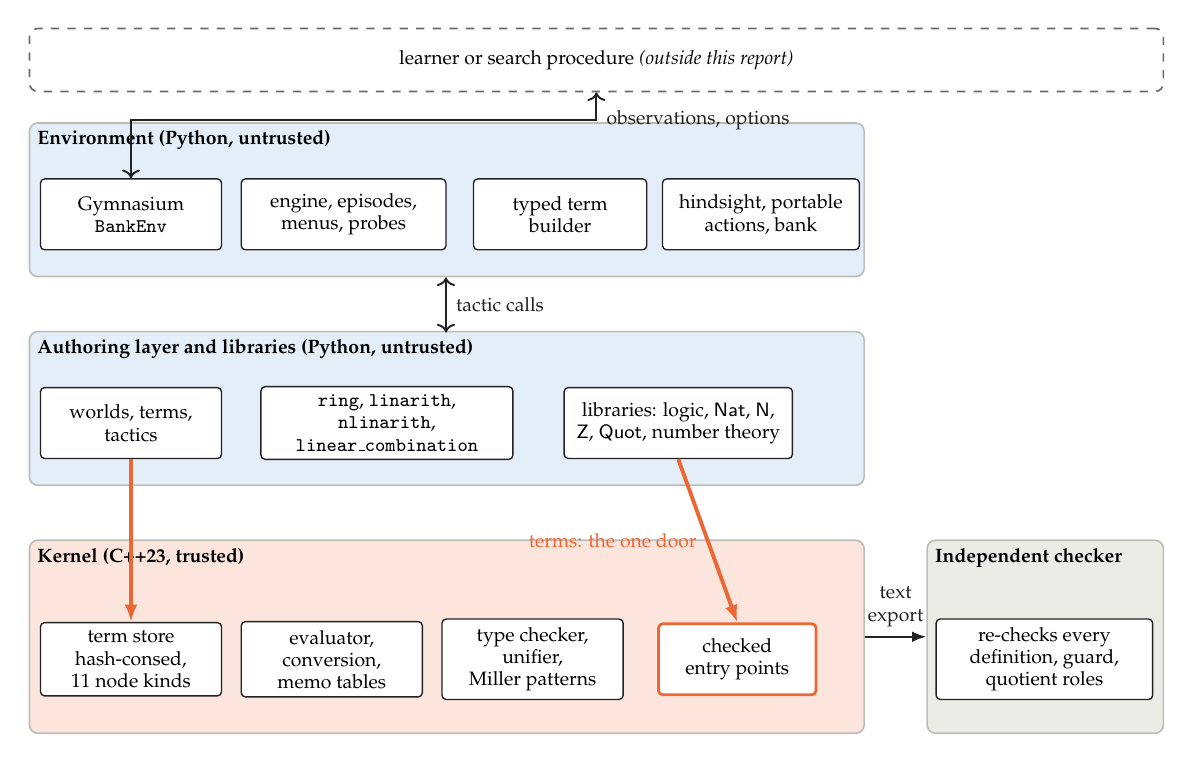
\begin{tikzpicture}[x=1cm,y=1cm,font=\footnotesize,
  box/.style={draw=ink, line width=0.5pt, fill=white, rounded corners=1.5pt, align=center, inner sep=3pt, minimum height=0.9cm, font=\scriptsize},
  band/.style={draw=rulegrey, line width=0.6pt, rounded corners=3pt},
  lab/.style={font=\scriptsize\bfseries, anchor=north west, inner sep=3pt},
  flow/.style={-{Latex[length=1.8mm]}, line width=0.7pt, color=ink},
  door/.style={-{Latex[length=2.2mm]}, line width=1.4pt, color=corange}]
  % bands
  \node[band, fill=trusted,   minimum width=10.6cm, minimum height=2.45cm, anchor=south west] (K) at (0,0) {};
  \node[band, fill=untrusted, minimum width=10.6cm, minimum height=1.95cm, anchor=south west] (A) at (0,3.15) {};
  \node[band, fill=untrusted, minimum width=10.6cm, minimum height=1.95cm, anchor=south west] (E) at (0,5.8) {};
  \node[band, fill=second,    minimum width=3.0cm,  minimum height=2.45cm, anchor=south west] (I) at (11.4,0) {};
  \node[draw=muted, dashed, line width=0.6pt, rounded corners=3pt, minimum width=14.4cm, minimum height=0.8cm, anchor=south west, fill=white] (L) at (0,8.15) {\scriptsize learner or search procedure \emph{(outside this report)}};
  % labels
  \node[lab] at (K.north west) {Kernel (C++23, trusted)};
  \node[lab] at (A.north west) {Authoring layer and libraries (Python, untrusted)};
  \node[lab] at (E.north west) {Environment (Python, untrusted)};
  \node[lab] at (I.north west) {Independent checker};
  % kernel boxes
  \node[box, minimum width=2.3cm] (k1) at (1.3,0.95)  {term store\\ hash-consed,\\ 11 node kinds};
  \node[box, minimum width=2.3cm] (k2) at (3.85,0.95) {evaluator,\\ conversion,\\ memo tables};
  \node[box, minimum width=2.3cm] (k3) at (6.4,0.95)  {type checker,\\ unifier,\\ Miller patterns};
  \node[box, minimum width=2.0cm, draw=corange, line width=1.0pt] (k4) at (9.0,0.95) {checked\\ entry points};
  % authoring boxes
  \node[box, minimum width=2.3cm] (a1) at (1.3,3.95)  {worlds, terms,\\ tactics};
  \node[box, minimum width=3.2cm] (a2) at (4.55,3.95) {\code{ring}, \code{linarith},\\ \code{nlinarith},\\ \code{linear\_combination}};
  \node[box, minimum width=2.9cm] (a3) at (8.25,3.95) {libraries: logic, $\Fam{Nat}$, $\Fam{N}$,\\ $\Fam{Z}$, $\Quot$, number theory};
  % environment boxes
  \node[box, minimum width=2.3cm] (e1) at (1.3,6.6)  {Gymnasium\\ \code{BankEnv}};
  \node[box, minimum width=2.6cm] (e2) at (4.0,6.6)  {engine, episodes,\\ menus, probes};
  \node[box, minimum width=2.2cm] (e3) at (6.75,6.6) {typed term\\ builder};
  \node[box, minimum width=2.5cm] (e4) at (9.3,6.6)  {hindsight, portable\\ actions, bank};
  \node[box, minimum width=2.75cm] (i1) at (12.9,0.95) {re-checks every\\ definition, guard,\\ quotient roles};
  % flows
  \draw[flow, <->] (L.south) -- ++(0,-0.35) node[right, font=\scriptsize] {observations, options} -| (e1.north);
  \draw[flow, <->] (E.south west) ++(5.3,0) -- ++(0,-0.7) node[midway, right, font=\scriptsize] {tactic calls};
  \draw[door] (a3.south) -- (k4.north) node[midway, left, font=\scriptsize, color=corange] {terms: the one door};
  \draw[door] (a1.south) -- (k1.north);
  % export to the second checker
  \draw[flow] (K.east) -- node[above, align=center, font=\scriptsize] {text\\ export} (I.west);
\end{tikzpicture}
\caption{Architecture.
  Orange: the trusted base, the kernel, whose checked entry points are the only way a declaration enters the environment (the heavy arrows).
  Blue: untrusted layers; they construct terms and can only submit them.
  Grey: the independent checker, a second implementation of the specification that reads the kernel's text export of an environment and re-checks every definition.}
\label{fig:arch}
\end{figure}

\begin{table}[t]
\centering\tabfont
\begin{tabular}{@{}lp{8.6cm}r@{}}
\toprule
component & role & lines\\
\midrule
kernel (C++23) & term store, evaluation, checking, unification, tactic core, bindings & \lockernel\\
frozen reference kernel & the previous generation, kept fixed as a point of comparison & \locrefkernel\\
authoring layer & worlds, terms, tactics, \code{ring}, \code{linarith}, \code{linear\_combination} & \locauthoring\\
libraries & logic, naturals, integers, quotients, number theory & \loclibdir\\
independent checker & second implementation of the specification & \locchecker\\
environment & engine, menus, probes, term builder, hindsight, recorder & \locenvdir\\
problem bank & 268 statements, reference proofs, statement audit & \locprobdir\\
Gymnasium and learning code & \code{BankEnv}; code of a first learner, not evaluated here & \loclearner\\
synthetic theorem generator & & \locsynth\\
experiment drivers & benchmarks, measurement scripts, pipeline for later runs & \locexper\\
tests (the gates) & & \loctests\\
mutation catalogue and driver & & \locmutants\\
tools, examples & & \loctools, \locexamples\\
\bottomrule
\end{tabular}
\caption{Size of the components in lines of source (Python, C++ and headers) in the files tracked by git at commit \mCommit.}
\label{tab:loc}
\end{table}

\subsection{The kernel}\label{sec:kernel}

\paragraph{Terms.}
Every node is interned in a pool of its kind, an open-addressing hash table with a finalising mix of the hash so that structurally related nodes do not cluster; structurally equal terms are the same handle (a tag and an index), and equality of terms is a comparison of integers \citep{filliatre06}.
Terms are therefore DAGs, and the cost of checking a proof is a function of its size as a DAG and not as a tree.
The values of the \shareValues\ definitions and theorems of the libraries have, together, \shareTree\ nodes counted as trees, whereas their types and values together consist of \shareDistinct\ distinct nodes, a factor of \shareRatio.
Each compound node carries precomputed facts (the range of loose bound variables, the set of free context variables, a saturating size, and whether it mentions a metavariable), which let instantiation and abstraction skip every subterm they cannot affect.
Bound variables are de Bruijn indices, so that a closed term has one representation, and variables of the context are de Bruijn levels, so that extending the context renumbers nothing \citep{debruijn72,mcbride04,chargueraud12}.

\paragraph{Environments and values.}
The evaluator of \cref{sec:conv} runs in persistent environments, singly linked lists with Myers' skew-binary jump pointers \citep{myers83,okasaki95}: extension is one allocation and indexing is logarithmic, and closures share their environments.
Values are copied in constant time through shared immutable sequences, and the neutral-term spines of a conversion are compared by identity before they are compared by content.
Reference counts are intrusive and released iteratively, since a chain half a million nodes long once overflowed the stack when it was freed recursively.

\paragraph{Memoisation.}
Four tables and a quick check sit in front of the evaluator, and each table is keyed so that a hit is a fact about the question asked.
The \emph{typing memo} records the type of a term of at least 16 nodes, keyed by the node, the typing context, the evaluation switches and the epochs of the tables it depends on; it is used only for terms without metavariables in contexts without metavariables, and not at all while constraints are pending.
A \emph{quick conversion} on syntax runs before the evaluator and can only answer ``yes'' (identical nodes, congruence, binders, one delta step, beta), within a budget of steps and depth; on a ``no'' or a give-up the evaluator decides.
Two tables remember pairs of shared constructor values and shared spines found convertible or unifiable after real work, and a fourth remembers the read-back of shared stuck values, which removes the exponential cost of failing on a DAG whose paths are all walked.
During the build of the libraries, \memoShare\,\% of typing queries are answered from the memo (\memoHits{} hits, \memoMisses{} misses), and the quick conversion settles \synSettled\ of the \synTried\ comparisons it is asked.
With a debugging switch on, \emph{every} answer taken from any table is re-derived with all tables bypassed and a step limit, and a mismatch throws; the gates run with it on.
No table stores a refusal, so a table can hide a bug only by answering ``yes'' wrongly, which is what the verification switch is for.

\paragraph{Resource control.}
Every function that can run long begins with a check that decrements a deterministic work counter (``fuel'') and compares the stack pointer with the thread's floor, and throws a typed exception when the counter is spent or the stack is nearly full.
Both exceptions are caught at the module boundary and turn a runaway computation into a refusal that names the cause; nothing else can be read from them, and no code path treats exhaustion as success.
The authoring default is $2\times10^9$ steps per call; the environment gives each kind of action its own, much smaller, budget, so that a probe that does not finish is reported as having run out of work and not as having been refused.
Conversions are nested at most 256 deep and proof-irrelevance checks eight deep, and beyond the bound the answer is ``not equal'' and ``not irrelevant''.
The work of the decision procedures that is done in Python before the kernel sees a term is counted too, in units of the same budget (\cref{sec:testing}, finding F90).

\paragraph{State is a value.}
A \emph{checkpoint} records the sizes of the node pools, of the table of globals, and the marks of the metavariable trail; \emph{rewind} truncates the pools back to those sizes, removes the interned entries of the nodes it discards, and undoes the assignments since the mark.
Its cost is proportional to what was allocated since the checkpoint.
This is what a probe uses: run an action, observe the goals it leaves, and rewind, so that a refused action leaves the kernel exactly as it was.
The Python layer keeps handles to kernel nodes in caches that refuse to store while a probe is open, since a handle stored across a rewind could name a node that no longer exists or, worse, another node that took its index.

\paragraph{Determinism.}
No result depends on a memory address: tables are keyed by indices and hashes of indices, and no iteration order of an address-keyed container reaches a result.
The same probe gives the same goals, and a whole run gives the same outcome digest on every repetition (\cref{sec:why}).

\subsection{The authoring layer and the libraries}\label{sec:authoring}

The authoring layer builds terms and drives the kernel's tactics; \emph{nothing in it is trusted}.
A \texttt{World} is one kernel with a name table.
Binders are written in higher-order abstract syntax (\texttt{w.pi(A, lambda x: B(x))}) and built in the locally nameless style: a bound variable is a fresh context variable while the body is built and is abstracted when the binder closes.
Declarations (\texttt{inductive}, \texttt{define}, \texttt{recursive}, \texttt{theorem}) go through the checked entry points of \cref{sec:trust}.
A proof is a script of tactics over named hypotheses (\texttt{intro}, \texttt{cases}, \texttt{induct}, \texttt{apply}, \texttt{rewrite}, \texttt{exact}, \texttt{ring}, \texttt{linarith}, and others); the script builds a term, and the term is submitted.

The libraries are built in stages, each on the last, entirely through this layer: logic and equality; unary naturals; binary naturals; the ring lemmas; quotients; the integers as the quotient of pairs of binary naturals; elementary number theory; an extension library; and the Olympiad-problem library.
\Cref{tab:libs} lists the stages.
A census of the \libGlobals\ declarations gives \censusInd\ inductive families with \censusCtor\ constructors, \censusDef\ definitions, \censusRec\ recursive functions, \censusThm\ theorems, the \censusQuot\ quotient constants and one axiom, \censusAxiomName\ (excluded middle, used by the number-theory library).

\begin{table}[t]
\centering\tabfont
\begin{tabular}{@{}lrrr@{}}
\toprule
stage (module) & declarations & build, run 1 (s) & run 2 (s)\\
\midrule
\libGroupRows
\midrule
total & \libGlobals & \libBuildA & \libBuildB\\
\bottomrule
\end{tabular}
\caption{The library chain, built from nothing by \ITP, on the machine of \cref{sec:why}: declarations added at each stage and the time to build it, in two independent runs.}
\label{tab:libs}
\end{table}

\subsection{The independent checker}\label{sec:indep}

A second checker, \texttt{indep\_checker}, re-checks the results.
It was written from the specification of \cref{sec:theory}, not from the C++ kernel, and built differently on purpose.
\begin{center}\tabfont
\begin{tabular}{@{}lp{5.2cm}p{5.6cm}@{}}
\toprule
 & kernel & independent checker\\
\midrule
language, size & C++23, \lockernel\ lines & Python, \locchecker\ lines (with its drivers)\\
variables & de Bruijn indices and levels & names, explicit capture-avoiding substitution\\
conversion & evaluation to a semantic domain, memo tables & weak-head normalisation, no caches\\
fixpoints & one layer on any argument & only on a constructor argument\\
$\eta$ & function $\eta$ & function $\eta$, in both directions\\
metavariables, $\sy{let}$ & supported & reported as unsupported\\
\bottomrule
\end{tabular}
\end{center}
It shares with the kernel only the \emph{input format}: the kernel's text export of an environment.
It re-implements the universe rule for products, the structural guard, the parameter analysis, the \textsc{Match} rule with the forcing of \cref{alg:force}, the elimination restriction, definitional proof irrelevance with its depth bound, and the validation of the quotient constants; for those it does not trust the labels the kernel puts on them.
It checks every definition and theorem of an environment (the value against the type), every recursive function against the guard, and every type; it does \emph{not} re-check the admission of inductive families (the positivity and universe conditions \textbf{A4} and \textbf{A5}), nor the unifier, which it does not need: an admitted term contains no metavariable.
Used on the libraries, it re-checks all \indGlobals{} globals in about \indCheckA\,s (after a load of \indLoadA\,s) and accepts every one; on the reference proofs of the problem bank it re-checks a sample (\cref{sec:why}).
It is slow and memory-hungry by design: it is a witness and not a tool of the inner loop, and a proof it cannot finish within its limits is reported as such and counted, and not as accepted.

The checker has found defects in the kernel, among them an unvalidated binder annotation in a lambda checked against a product (F21); the comparison has also exposed disagreements that were defects of the checker (F27: the checker had no function $\eta$) and one defect of both, a branchless match on an inhabitant of an opaque type constant, which each accepted as a proof of anything until a test of quotients tried an inhabited opaque type (F26, a soundness defect, fixed in both).
The last case is the lesson of the apparatus: two implementations of one specification agree on whatever the specification gets wrong.

\subsection{The environment}\label{sec:env}

The environment is the Python layer of \code{src/python/environment} together with the problem bank (\locenvdir{} and \locprobdir{} lines, \cref{tab:loc}).
It is untrusted (\cref{sec:trust}): it asks the tactic layer to construct terms, and what an episode ends with is a proof term that the kernel checks against the statement.
Its job is to make three things operations of a library call and not services of a process: to read a state as data, to try an action and take it back, and to list what can be done.

\paragraph{Goals and steps.}
A \emph{goal} is a target and the types and names of its hypotheses, all of them kernel handles.
Terms are hash-consed, so two searches that reach the same goal by different routes reach the same object, and a goal has a key under which a search can recognise it.
A goal can be read as arrays (node tags, scalars, child pointers, roots, heights) by a consumer that wants the term structure, or as a token sequence by one that wants a sequence.
A \emph{step} is an \emph{action}, a kind and its arguments (\cref{tab:actions}), applied to the first open goal.
After every step the goals it leaves are \emph{settled}, in the same way in a probe as in a replay: a goal that a hypothesis or reflexivity closes is closed, and the quantifiers and implications at the head of a goal are introduced, so that no step is spent on either.

\begin{table}[t]
\centering\tabfont
\begin{tabular}{@{}l>{\raggedright\arraybackslash}p{3.3cm}>{\raggedright\arraybackslash}p{6.4cm}@{}}
\toprule
kind & argument & effect\\
\midrule
\multicolumn{3}{@{}l}{\emph{First language: the agent chooses an action from a finite menu (kinds 0--11)}}\\
\code{INTRO} & --- & introduce the first binder (needed only when automatic introduction is off)\\
\code{CASES}, \code{INDUCT} & a hypothesis, and hypotheses to generalise & case analysis, induction\\
\code{APPLY} & a lemma or hypothesis of the menu & apply it, where the goal determines its data arguments\\
\code{REWRITE} & a lemma or hypothesis, a direction & rewrite at the first instance\\
\code{RING}, \code{LINARITH}, \code{NLINARITH} & --- & the decision procedures of \cref{sec:certificates}; \code{NLINARITH} multiplies pairs of hypotheses\\
\code{BY\_CONTRA} & --- & classical: assume the negation, prove \code{False}\\
\code{INTERVAL\_CASES} & a variable and its two bounds & split an integer variable bounded on both sides\\
\code{INSTANTIATE} & terms of the goal's pool & \code{have h := H t$_1$ \ldots}\\
\code{USE} & a term of the pool & the witness of an existential goal\\
\midrule
\multicolumn{3}{@{}l}{\emph{Second language: the arguments are said, one typed choice at a time (kinds 12--20)}}\\
\code{CLAIM} & a statement & \code{have h : s}; two goals, the statement and the goal with \code{h}\\
\code{REFINE} & a term with holes & \code{exact}; each hole is a proposition left as a goal\\
\code{APPLY\_WITH}, \code{REWRITE\_WITH} & a source and the data arguments the goal does not determine & apply, rewrite; the unifier finds the rest\\
\code{REWRITE\_AT} & as \code{REWRITE\_WITH}, and a hypothesis & rewrite inside a hypothesis\\
\code{FORWARD} & a source and argument slots & \code{have h := source s$_1$ \ldots}\\
\code{INDUCT\_WITH} & a library principle, its other arguments, a variable & induction by a chosen principle; the motive is read off the goal\\
\code{INJECT} & a hypothesis $c\,\vs{a}=c\,\vs{b}$ & the equations $\vs{a}=\vs{b}$\\
\code{LINCOMB} & hypotheses and coefficient terms & \code{linear\_combination}, closed by \code{ring}\\
\bottomrule
\end{tabular}
\caption{The twenty-one kinds of action.
  The numbers are part of the data format of recorded proofs.}
\label{tab:actions}
\end{table}

\paragraph{Probes.}
A \emph{probe} takes a checkpoint (\cref{sec:kernel}), runs an action on a one-goal copy of the goal, reads off the goals the action leaves, and rewinds: every node allocated in the meantime is reclaimed and every assignment of a metavariable undone.
Its outcome is one of four statuses: \code{ok}, with the goals the action leaves; \code{refused}, when the tactic or the kernel said no, when the goal came back unchanged, or when the goals it leaves are not independent; \code{fuel}, when the work budget ran out; and \code{bug}, when something other than a refusal went wrong.
Taking an action probes it first, so that an action that does not apply raises an error and changes nothing, and a learner or a search can try as many actions as it likes at the price of the probes.

\paragraph{Budgets.}
Every probe runs under a deterministic work budget that depends on the kind of action: $5\times10^6$ steps by default, $5\times10^7$ for \code{RING}, \code{LINARITH}, \code{INTERVAL\_CASES} and \code{LINCOMB}, and $1.5\times10^8$ for \code{NLINARITH}.
The decision procedures compute in Python before the kernel sees a term, and they spend the same units: the normaliser of \code{ring} counts its work before it allocates the memory the work stands for, and stops at one fiftieth of the kernel budget of the call.
Listing a menu runs kernel calls as well (the normal forms of candidate facts and of the goal), and each is bounded by $5\times10^6$ steps, a candidate fact of \code{INSTANTIATE} by one fiftieth of that.
A spent budget is reported as \code{fuel} and never as a refusal, since a larger budget might succeed; a learner should not be taught that an action is wrong because it was slow.
The three places where such a bound was missing (the assembler of terms, the listing of a menu, the normaliser of \code{ring}) were found by long runs, two of which were killed by the operating system, and not by any gate; each is now pinned (findings F86, F87, F90 of \cref{sec:testing}).

\paragraph{The first language.}
Twelve kinds of action take their arguments from a finite menu.
A menu is a list of actions together with the table of lemmas and hypotheses they name; the lemmas offered for \code{APPLY} and \code{REWRITE} are those that a library index says can match the goal, and for \code{APPLY} those whose data arguments the goal determines.
The two kinds that carry terms, \code{INSTANTIATE} and \code{USE}, take them from a deterministic pool of small well-typed terms built from the variables and numerals of the goal.
A menu is a finite, ordered, deterministic list, so that a policy can score it and a search can enumerate it.

\paragraph{The second language and the typed term builder.}
A finite menu cannot offer an arbitrary term: a witness, an intermediate statement, an instance of a lemma at chosen arguments.
Nine further kinds therefore take \emph{codes}, tuples of tokens of a \emph{typed term builder}.
A term is built in prefix order, one choice per step, and at each step the builder offers only the tokens that keep the term well typed: a variable of the context applied to $k$ arguments, a global applied to $k$ arguments, a numeral of the type at the hole, a lambda, a universal quantifier, an implication, a sort, a term of the pool, or (for \code{REFINE}) a proposition left open as a goal.
A head takes the arguments its type needs to reach the type at the hole, except those that the expected type already determines (the implicit carriers), so that a statement is said without the noise that a fully applied term would carry.
A policy that chooses among the offered tokens cannot say an ill-typed term; the gates check this by random walks over the choices, and the kernel checks the finished term again.
The builder says and builds back the terms of the proofs of the libraries (\code{encode}, \code{build}) with one exception that it reports and does not hide: a term with \code{match} or \code{let} cannot be said, which concerns two proofs of the libraries and the statement of functional extensionality.
A lemma above the engine's premise limit cannot be said either.

\paragraph{Premises and regimes.}
An attempt may use only the globals that its \emph{premises} allow, a number: a theorem is attacked with the library that precedes it, and the problems of a bank do not see each other's solutions.
Two regimes follow from the lemmas that were written for a problem.
In the \emph{prefix} regime every global before the theorem is on offer, the problem's own helpers included, which measures how well an agent uses a good lemma; with its helper on the menu a problem can be a single action.
In the \emph{strict} regime the helpers written for the problem are hidden, from the menu and from the builder alike, so that the problem tests whether the ideas can be found.
A reference proof must be self-contained for the strict regime (it proves its lemmas inline), and this is checked by replaying the proof with the helpers hidden, not assumed.
An episode carries its own premises, so that episodes of different regimes interleave on one engine.

\paragraph{Portable actions and the recorder.}
An action can be written as plain data, with no kernel handle and no index into a menu: a lemma is named by its identifier in the world, a hypothesis by its level.
A recorded proof can therefore be stored in a file, sent to another process and replayed in a fresh engine; malformed data raises the environment's error and nothing else.
The \emph{recorder} turns authored tactic proofs into such sequences.
It runs a library with every tactic call logged as a tree, translates each call into candidate plans of engine actions, keeps the first plan whose probe leaves as many goals as the author's call left, carries it out, and finally has the kernel check the proof the engine built.
All but six of the 459 recorded proofs of the libraries replay in this way; the six, named in the gate S40 together with their reasons, are two proofs whose terms contain a \code{match} or compute only, two authored inductions whose hypothesis the engine does not have, and two applications whose goals the engine settles by itself.
A translation that is wrong makes a replay fail, and cannot produce a false theorem.

\paragraph{Hindsight.}
A failed attempt contains theorems that \emph{were} proved: a case that closed, a fact that an action derived.
With tracking on, an episode keeps its proof tree and returns these as new standalone problems with proofs, by analogy with relabelling a failed trajectory by what it did achieve \citep{andrychowicz17}.
Because the engine settles goals, the statement of a sub-tree as the agent saw it is not always the statement that a replay proves; an example is therefore returned only after it has been replayed from its own data in a fresh engine and checked by the kernel, and the candidates that cannot be made exact are dropped and counted by reason.
Hindsight is a feature of the data, not of the logic: the examples are as sound as the replay that produced them.

\paragraph{The problem bank.}
A \emph{problem} is a theorem of one deterministic world plus what a dataset needs to know about it: the problem in words, its source, topics and a level from 1 to 5, whether it asks for a proof, for an answer (``determine all'': the answer is part of the statement, an equivalence with the solution set) or for an example, a reference proof, and an executable reading of the intended meaning.
The bank has \bankProblems{} problems from AMC, AIME, IMO, ISL and APMO papers, classical exercises, and graded problems written for the bank, in a world of \bankGlobals{} globals (the libraries and the statements).
\proofsProved{} of them have a reference proof that is kernel-checked and replays through the action language; the remaining \statementOnly{} are \emph{statement-only}: the formal statement is the task, and an agent that proves one is checked by the kernel all the same.
The reference proofs total \proofsTotalActions{} actions (median \proofsMedian, 90th percentile \proofsNinety, longest \proofsMax).
The kernel establishes that a proof proves its statement; that the statement says what the problem says is a separate question.
A statement is therefore read back from its kernel term into a small syntax tree and evaluated on integers, over windows of small values, against an intended meaning that the person who formalised the problem wrote as a Python predicate; the meaning of each symbol of the library is written down once, in a few dozen lines to audit, and compared with the library's definition.
Mutated statements (a swapped relation, a dropped hypothesis) serve as negative controls that the comparison must notice or explain.
A check on a window is a check of meaning on small values and never of truth.
For the statement-only problems, an exhaustive search on a larger range, written from the problem and not from the formal statement, supplies evidence for the claim itself.
A statement audit reports, for every problem, the checks made and the cautions where the evidence is weaker.
No second reader's verdict is recorded yet, and a misreading of the English that the statement and its executable reading share is invisible to every check (\cref{sec:limits}).
The splits into training, development and test problems are by family and not by problem (the two parts of one olympiad problem, or a statement and its restatement, belong together), and the split of a family is a pure function of its key, so that adding problems moves none.

\paragraph{The Gymnasium interface.}
\code{BankEnv} wraps the engine for the bank as a Gymnasium environment \citep{towers24,brockman16} at the level of the policy's \emph{decisions}.
One episode is one proof attempt on the first open goal.
To act, the agent answers the engine's questions in turn (the kind of action, the lemma, the hypothesis, then the next token of a term), each among the \emph{options} that the engine offers at that point; when the last question is answered the action is probed and, if it applies, taken.
The observation is a dictionary of integer arrays: the goal as token identifiers with a segment and a hypothesis index for each token, the number of hypotheses and goals left, the budget left, the overlap of each global's symbols with the goal, the kind of decision, the tokens of the type of the term being said, and the options as integer rows with a count and a legality mask.
The action space is \code{Discrete(1024)}, the index of an option; an illegal index raises an error, or with \code{illegal='penalize'} loses the decision.
The reward is $1$ when the finished proof has been checked by the kernel, and an optional penalty per action or refusal; an episode is truncated after 60 actions (taken or refused) or 600 decisions, both configurable.
An episode may start from any closed statement given as portable data, which is how hindsight examples are used.
There is no text interface anywhere in this chain.

\subsection{Testing}\label{sec:testing}

The architecture localises what must be right.
Only the kernel can accept a false statement; the independent checker is a witness whose disagreement is information; everything else can lose a proof but not make one.
The tests are accordingly aimed at the kernel and at the boundary around it, and the rest of the apparatus protects usefulness (an action that should apply, a probe that returns).
This subsection describes the apparatus and states what each part shows.
The numbers are those that the named gates printed when we ran them for this report (\code{measure\_gates.py}), at commit \mCommit{} on the machine of \cref{sec:measure}; all \gatesAll{} gates were then run once more, as a whole (\cref{app:gates}), and the logs of both runs are in the supplementary material.

\paragraph{Gates.}
A \emph{gate} is a self-contained script that exits 0 and prints no failure if and only if the property it protects holds.
There are \gatesAll{} (\gatesDefault{} by default; the others need the machine-learning libraries, the repository, or the synthetic theorem generator), organised by what they protect: the kernel against a frozen reference, its soundness, boundaries and performance guards, quotients, proof irrelevance and the work budget; the libraries and decision procedures; the environment; the problem bank; and the repository itself.
The gates of the default set can also be run with every answer that the kernel takes from a sharing table re-derived with the tables bypassed (\code{ITP\_VERIFY\_MEMO=1}, \cref{sec:kernel}); this about doubles their time and is how the memo tables are tested.

\begin{table}[t]
\centering\tabfont
\begin{tabular}{@{}>{\raggedright\arraybackslash}p{3.3cm}>{\raggedright\arraybackslash}p{4.4cm}>{\raggedright\arraybackslash}p{5.1cm}@{}}
\toprule
apparatus & what is compared or attempted & result at this commit\\
\midrule
lockstep against the frozen reference kernel (S2, harness) &
  random typed terms with \code{match}, corpora of inductive families and recursive functions, random terms for normal forms, conversion and typing; both kernels must give the same verdict &
  \lockMatchTerms{} well-typed and \lockIllTyped{} ill-typed matches, \lockDepChecked{} dependent-typing checks, \lockAdmission{} admission and \lockGuard{} guard cases, \harnessComparisons{} comparisons on \harnessTerms{} terms; no disagreement\\
self-consistency oracle &
  random tactic scripts in five distributions; after each tactic the partial proof must type-check against the statement &
  \oracleCompleted{} proofs completed, \oracleVerified{} verified; no unattributed failure\\
independent checker (S8) &
  random scope-aware mutations of valid proofs, judged by the kernel and by the checker &
  \indepMutated{} mutated proofs: both accept \indepBothAccept{}, both reject \indepBothReject{}, no verdict differs\\
soundness canaries (S15, S16) &
  a blind random generator of proof attempts on statements that are \emph{false}; the same generator on true statements as a check on its power &
  classical axioms: \canaryClassAttempts{} attempts at \canaryClassFalse{} false statements, none completes; \canaryClassPowerOk{} of \canaryClassPower{} attempts at true ones complete, all verified. Quotients: \canaryQuotAttempts{} attempts, none completes; \canaryQuotPowerOk{} of \canaryQuotPower{}, all verified\\
boundary (S19) &
  malformed or hostile calls through the Python API: nothing may crash, hang, or be accepted &
  \boundaryCases{} cases pass; \boundarySeeds{} seeds of \boundaryCallsSeed{} random calls, each in a child process\\
\bottomrule
\end{tabular}
\caption{Parts of the test apparatus aimed at the kernel and what they printed.
  A random generator that completes nothing is also what a toothless generator does, so each canary is paired with a run of the same generator on true statements, which must complete and verify a minimum number of proofs.}
\label{tab:testing}
\end{table}

\paragraph{Lockstep against a frozen reference.}
The previous generation of the kernel (absolute universe levels, variables as levels) is kept byte-for-byte, with its checksums pinned by a gate, and the same random inputs are given to it and to the hybrid kernel.
Where the hybrid kernel is deliberately stricter, or fixes a defect of the reference, the gate says so explicitly (for instance F19; \cref{tab:findings} counts the findings by layer).
The lockstep comparison tests that a rewrite of the representation preserved the behaviour; it says nothing about a defect that both kernels share.

\paragraph{A second checker.}
\Cref{sec:indep} describes the checker; \cref{tab:testing} gives its agreement with the kernel on mutated proofs.
The mutations (a variable replaced by another in scope or by a constant, a constant replaced, a universe level shifted, the two parts of an application exchanged, a binder annotation replaced, two branches of a match exchanged, the decreasing argument of a fixpoint moved) produce mostly ill-typed terms, which is what the comparison needs: a checker that accepts a term that the kernel rejects, or conversely, is a finding.

\paragraph{Canaries.}
If a rule added to the trusted base made it inconsistent, a blind generator of tactic scripts would eventually complete and verify a proof of a false statement.
The canaries of the two additions that put the base at risk (the classical axioms, in the world in which \code{Type 0} is \code{Prop}, and the quotient constants) throw random attempts at statements that are false in the intended model.
That none completes is evidence of the kind that testing gives: of the absence of a cheap attack, not of consistency.

\paragraph{Falsification through the environment.}
A fuzzer drives the tactic layer, the unifier and the kernel's final check through the environment: it generates statements about the natural numbers or the integers, decides by evaluation which are true (true ones by equality-preserving rewrites of a random term, false ones by a small perturbation of a true one), and runs the search on each.
It classifies the outcomes as \code{REJECTED} (a finished proof that the kernel then refused: a defect of the tactic layer or the unifier), \code{UNSOUND} (a proof of a statement that is false at some point: a defect of the kernel, which should be impossible) and \code{ERROR} (any other exception out of the engine).
A rejection is always a bug, since it is a disagreement between two layers; the first two defects found this way were in the tactic layer and the unifier.
The campaign that collects its results into one folder (\code{make soundness}) takes hours, was not run for this report, and its output is not quoted.

\paragraph{Mutation testing.}
A test suite that has never failed has not been shown to test anything.
The mutation catalogue holds \mutTotal{} mutants, each of which re-breaks one rule of the system in an isolated copy of the tree, and the gates must fail on it.
Of these, \mutKernel{} mutate the C++ kernel (\mutKernelHeader{} the header, \mutBindings{} the bindings), \mutChecker{} the independent checker, \mutTactic{} the tactic layer and the decision procedures, \mutLibrary{} the libraries, and \mutEnv{} the environment, the action language, the term builder and the recorder.
A mutant that no gate catches is a gap in the tests unless it is one of the \mutEquiv{} documented equivalents, for which no input can tell the mutant from the original.
Its limits are part of the result.
The catalogue was run series by series as the code it refers to was written; the more recent additions were run against the gates that pin them; we report no single pass of all of it against the final commit, which takes many hours.
There are no mutants of the same kind for the problem-set modules, the learner, the generator or most of the experiment pipeline, whose gates rely on fixtures with hand-worked expectations and on tamper tests, and have not been shown to bite by mutation.
Some mutants are known to survive (one of the recorder's, whose fallback nothing exercises), and twenty environment mutants whose anchors were repaired by hand after a refactoring were not run again.
The mutants are written by the author of the code, so they measure the tests against the faults that the author can imagine.

\paragraph{Sanitizers.}
The evaluator owns its memory by hand (intrusive reference counts, single-allocation sequences, a trampoline that frees deep chains iteratively), and a bug there would not show as a wrong answer but as a use after free that the functional gates cannot see.
The kernel can be built with AddressSanitizer and UndefinedBehaviorSanitizer, and the gates run under it.
For this report we ran \sanGates{} of the \sanDefault{} gates that the tool selects by default (the lockstep, soundness, quotient, irrelevance, conversion, tactic and independent-checker gates of the kernel and the differential harness) with the sanitizers on, and all pass, in \sanSeconds{} seconds.
The tool leaves out \sanLeftOut{} further gates, because they limit the address space, which the sanitizer cannot start under, or carry time limits meant for an unsanitized build, or recurse a gigabyte deep, which the sanitizer reports as a false positive.
The remaining gates of the default set, the long ones of the libraries, the environment and the bank, were not run under the sanitizers.
Leak detection is off, since the Python interpreter itself leaks at exit; the evaluator's leaks are checked separately, by a standalone driver, which we did not run for this report.

\paragraph{Faults in the tools that make evidence.}
The numbers of an experimental report come from tools, and a test written together with the code it checks tends to check what the code does and not what it must do.
Single-line faults were therefore injected into each of \toolCount{} tools (the soundness folder, the statement audit, the number checker, the record of which code produced a result, the digest of the code, and the runner of these faults itself), \toolFaults{} faults in all, and the gate section written for the tool must fail for every one.
Of the first 172 faults, 21 got past the tests that had been written for the tool, among them stages that reused a saved result made for other code and would have made a folder say \code{CLEAN} about code it had never looked at (finding F88); all \toolFaults{} are now caught.

\paragraph{The log of findings.}
Every defect found while building the system, by a gate, a mutant, the second checker, a long run or a reading, is recorded in a log with its status and the test that fails without the fix.
It holds \findNumbers{} numbered findings (\findRows{} rows; the second, F2, has two parts).
Of the rows, \findFixed{} are fixed and pinned by a test that fails without the fix, \findConstruction{} are removed by the construction of the hybrid representation, \findMitigated{} are mitigated with the root cause open, \findPartial{} is partial, \findDocumented{} are documented design consequences or hazards, and \findOpen{} are open (\cref{sec:limits}).
The author tagged each row, when it was written, with the layer in which the defect lived and the effect it could have had; \cref{tab:findings} counts them (a row with two layers counts in both).

\begin{table}[t]
\centering\tabfont
\begin{tabular}{@{}llrp{6.2cm}@{}}
\toprule
layer & trust & rows & examples\\
\midrule
kernel & trusted & \findKernel & a lambda checked against a product never validated its binder annotation (F21); evaluation unfolds a fixpoint on a neutral argument (F23); conversion is incomplete on stuck matches (F28); work unbounded (F30)\\
independent checker & witness & \findChecker & no function $\eta$ (F27); a branchless match on an opaque type constant accepted (F26)\\
tactic layer, unifier, libraries & untrusted & \findTactic & \code{apply} accepted a solution of the wrong type for a metavariable (F25); a work bound missing in \code{ring} (F90)\\
environment: engine, builder & untrusted & \findEngine & unbounded kernel calls while listing a menu (F87) or assembling a term (F86)\\
bank, recorder, hindsight, generator & untrusted & \findData & statements, duplicated or misleading data; exactness of hindsight (F72)\\
training and experiment pipeline & untrusted & \findPipeline & estimates, documents, the record of the code\\
tests and tooling & --- & \findTooling & the mutation driver was vacuous after a reorganisation: every mutant looked caught (F71)\\
\bottomrule
\end{tabular}
\caption{The \findRows{} rows of the log of findings by the layer in which the defect lived.
  Three rows record trusted code that accepted what it must refuse (\findAcceptsIds): the first is in the frozen reference kernel (the hybrid kernel is stricter), the second was found by the independent checker, and the third, a soundness defect found while designing the quotient gate, was in the kernel and in the checker.
  All three are fixed and covered by tests that fail without the fix.}
\label{tab:findings}
\end{table}

\paragraph{What the lessons are.}
Four findings are lessons about the apparatus and not about the logic.
\emph{Two implementations of one specification agree on whatever the specification gets wrong} (F26): a branchless \code{match} on an inhabitant of an opaque type constant was accepted as a proof of anything by the kernel and by the checker, because both read the family of a type from the same unwritten assumption, and it was found by a test of quotients that for the first time inhabited an opaque type.
\emph{A check that can fail for reasons of infrastructure needs a baseline that runs in the same infrastructure} (F71): after a reorganisation, the copy of the tree in which the mutation driver runs a mutant lacked a directory, every gate crashed on an import, every mutant was reported as caught, and the baseline, which ran in the original tree, could not show it; the giveaway was a mutant ``caught'' by a seventy-second gate in no time.
\emph{A work bound must cover every computation that precedes the kernel} (F86, F87, F90): all three were found by the first long run of a component that the gates had run only briefly.
\emph{Tests written with the code check what the code does} (F88), which is why the tools that make evidence have faults injected into them.

\paragraph{What the testing shows and does not show.}
The kernel has been compared with an earlier kernel and with an independently written checker on large numbers of generated and mutated inputs, attacked with blind generators on false statements, built with sanitizers, and mutated; every defect so found is recorded.
None of this proves the kernel sound.
The two checkers share one specification, and a defect of the specification is invisible to both; the generators sample distributions that the author chose; the mutants are the faults that the author imagined; and the lockstep comparison is blind to what the two kernels share.
The statement of a theorem lies outside the chain altogether.
Soundness is tested here and not proved, and we make no claim of being more trustworthy than any other kernel.

\section{Using the system}\label{sec:usage}

\ITP\ is used as a Python library.
There is no surface language and no command-line prover: a definition, a tactic script and a query are Python, and a proof is a program that builds a term and submits it.
This section shows the system in use.
Each listing was run for this report (by \code{run\_listings.py} of the supplementary material), and the output printed under it is the output of that run.
The first two lines of every listing, which set up the module search path, are omitted here and are in the files.

\subsection{Setting up}\label{sec:setup}

The kernel needs a C++23 compiler (it uses \code{std::expected}); the measurements of this report were made with \mCompiler.
Python 3.13 with \code{numpy}, \code{scipy} and \code{nanobind} runs the kernel, the libraries, the tactics and the gates; PyTorch and Gymnasium are needed only by the learner and by the Gymnasium wrapper of the environment, and Matplotlib only by the figures of the experiment report.
From the root of the repository:
\begin{lstlisting}[style=out]
python3 -m venv .venv && source .venv/bin/activate
pip install "numpy>=2.5" "scipy>=1.18" "nanobind>=3.1"
make kernel         # builds the kernel and the frozen reference kernel
make gates-quick    # six kernel gates and the first example
\end{lstlisting}
On the machine of \cref{sec:measure}, building both kernels from scratch took \kernelBuildS\,s and \code{make gates-quick} \gatesQuickS\,s.

\subsection{A theorem, a decision procedure, and a refusal}\label{sec:use-prove}

\Cref{lst:prove} defines a function by structural recursion, proves a theorem about it by induction, closes a polynomial identity with \code{ring}, and then tries two things that must fail.
A \emph{world} is a kernel together with a name table; \code{nat\_lib.build\_nat()} returns one holding the library of unary naturals.
\code{w.recursive} submits the function to the kernel, which checks that the recursion is structural; \code{w.prove} runs a tactic script over named hypotheses, extracts the finished term, and hands it to the kernel's checked entry point of \cref{sec:trust}, and only then does the theorem exist in the world.
The false identity is refused by \code{ring} with the two normal forms in the message; the forged proof of $0=1$ never reaches the world, because the kernel checks it against the statement and finds that \code{Zero} and \code{Succ Zero} are different constructors.
The independent checker then re-checks every global of the world, and the audit reports the axioms and quotient constants that a theorem depends on (here none).

\lstfile[firstline=3]{A recursive function, an inductive proof, \code{ring}, and two refusals.}{lst:prove}{listings/ex_prove.py}
\lstinputlisting[style=out]{listings/ex_prove.out}

\subsection{Integers, \code{linarith} and \code{nlinarith}}\label{sec:use-int}

The integers are a library like any other: a quotient of pairs of binary naturals with every law proved (\cref{sec:authoring}).
In \cref{lst:int}, \code{ring} proves a polynomial identity over $\Z$; \code{linarith} finds non-negative multipliers by an exact simplex and the kernel checks that the weighted sum of the hypotheses and the negated goal is a negative constant, by \code{ring}; \code{nlinarith} adds products of hypotheses and squares and accepts a hint, here a proof of $0\le(x-y)^2$.
A claim that does not follow is refused with the reason.
Because the integers are built on the quotient, the audit of \code{am\_gm} reports the five quotient constants and no axiom: the trusted base of a statement about integers includes the rule $\kappa$ of \cref{sec:quot}, and this is visible.

\lstfile[firstline=3]{Integers: \code{ring}, \code{linarith}, \code{nlinarith}, a refused claim, and an audit.}{lst:int}{listings/ex_int.py}
\lstinputlisting[style=out]{listings/ex_int.out}

\subsection{An episode in the environment}\label{sec:use-env}

\Cref{lst:env} puts the same theorem to the environment instead of to a tactic script.
An \code{Engine} serves one world; an \code{Episode} is one proof attempt on a statement, with the premises it may use.
The menu lists the legal actions of the first open goal; an action that does not apply is refused and changes nothing; \code{INDUCT} is probed, taken, and the settling of the goals closes the base case by computation, leaving one goal with its induction hypothesis.
The last lines run the blind search of the environment, iterative deepening over the menus with a budget of probes; the proof it returns has been replayed on a live proof and checked by the kernel, so a wrong search can only fail.

\lstfile[firstline=3]{An episode: goal, menu, a refused action, an induction, and a blind search.}{lst:env}{listings/ex_env.py}
\lstinputlisting[style=out]{listings/ex_env.out}

\subsection{As a Gymnasium environment}\label{sec:use-gym}

\Cref{lst:gym} loads the problem bank and plays random legal options on one problem.
The observation is a dictionary of integer arrays (here only the shapes of three of them are printed), and every question the environment asks, here the kind of action, comes with a mask of its legal options.
Random play over fifty decisions assembles four actions, of which the probe takes two and refuses two; a false statement could not be proved by any sequence of decisions, because the kernel checks the finished proof.
Loading the bank builds a world of \bankGlobals{} globals in about \bankWorldSec{} seconds and, with PyTorch loaded, \bankRSSTorch{}~GB of memory (\cref{sec:why}).

\lstfile[firstline=3]{The problem bank as a Gymnasium environment; random play over legal options.}{lst:gym}{listings/ex_gym.py}
\lstinputlisting[style=out]{listings/ex_gym.out}

\subsection{Checking, auditing, and reproducing}\label{sec:use-check}

\Cref{tab:commands} lists the commands that check the system itself and what each establishes.
The independent checker and the audit of \cref{lst:prove,lst:int} are also available on a whole world: \code{recheck\_world} of the module \code{recheck} exports the kernel's environment and re-checks every global, and \code{SecondOpinion} of the same module builds the checker's environment from the globals that a given set of terms needs, in seconds instead of a minute, and refuses (fails closed) a term that mentions anything else.
A reference proof is replayed and judged in the same way (gates S47, S50).
The measurements of \cref{sec:why} are reproduced by the scripts of the \code{preprint/} directory of the artifact (\cref{sec:conclusion}); every number of the text is read from their output.

\begin{table}[t]
\centering\tabfont
\begin{tabular}{@{}>{\raggedright\arraybackslash}p{4.1cm}>{\raggedright\arraybackslash}p{7.4cm}r@{}}
\toprule
command & what it establishes & time\\
\midrule
\code{make gates-quick} & the build works: six kernel gates and an example & \gatesQuickS\,s\\
\code{make gates} & the \gatesDefault{} default gates: kernel, tactics, environment, bank, contest proofs & 45\,min\\
\code{make gates-all} & all \gatesAll{} gates, including the learner's, the repository's and the generator's & \fullGatesWallMin\,min\\
\code{ITP\_VERIFY\_MEMO=1} \code{make gates} & the same, with every answer taken from a sharing table re-derived with the tables bypassed & about twice as long\\
\code{make mutants-check} & each of the \mutTotal{} mutants and \toolFaults{} tool faults still applies to the code it re-breaks & seconds\\
\code{python3 mutants/mutate.py} \textit{prefix} & the gates fail on every mutant whose name begins with the prefix & minutes to hours\\
\code{make sanitize} & the gates of the default set that can run under AddressSanitizer and UndefinedBehaviorSanitizer (\sanGates{} of \sanDefault) & \sanSeconds\,s\\
\code{make dataset-verify} & every recorded proof and sub-theorem of the dataset replays in a fresh engine and is kernel-checked & 25\,min\\
\code{make audit} & the audit of the bank's statements against their intended meaning, with a sheet for second readers & minutes\\
\bottomrule
\end{tabular}
\caption{Commands that check the system and what they establish.
  Times are on the two-core machine of \cref{sec:measure}; those of the quick gates, of all the gates and of the sanitizer run were measured for this report, and the others are those given by the repository's documentation.}
\label{tab:commands}
\end{table}

\section{What the design buys, and how it differs}\label{sec:why}

\Cref{sec:impl} describes the design; this section says what it is for, measures what it costs, and positions it among other systems.
It contains no result of learning.
Every claim about what a learner \emph{gains} is a claim about the properties of the interface; whether a particular learner profits is an empirical question that this report does not answer.

\subsection{What a learning loop needs, and what the design provides}\label{sec:properties}

A learning system uses a proof assistant in two ways: as a \emph{judge} of finished proofs, whose verdict is the training signal, and as an \emph{environment} that is called very many times.
\Cref{tab:properties} lists six properties of the design that bear on these roles, the mechanism behind each, and what we measured at this commit (\cref{sec:measure}).

\begin{table}[t]
\centering\tabfont
\begin{tabular}{@{}>{\raggedright\arraybackslash}p{3.1cm}>{\raggedright\arraybackslash}p{4.7cm}>{\raggedright\arraybackslash}p{4.7cm}@{}}
\toprule
property & mechanism & measured (\cref{sec:measure})\\
\midrule
a verdict that the proposer cannot influence, cheap enough to be asked for every finished proof &
  one checked entry point (\cref{sec:trust}); a second checker as a witness (\cref{sec:indep}) &
  kernel check of a reference proof: median \chkKernelMedianMs\,ms, longest \chkKernelMaxS\,s; the \kerDecls{} declarations of the libraries in \kerRecheckA\,s\\
trying an action and taking it back &
  checkpoint and rewind in time proportional to the allocation (\cref{sec:kernel}); probes (\cref{sec:env}) &
  median probe \probeMed\,ms, 99th percentile \probeNinetyNine\,ms; a checkpoint--rewind pair \rewPairNsA\,ns\\
actions that are well formed by construction, and no text in the loop &
  menus; the typed term builder (\cref{sec:env}) &
  one decision of the Gymnasium interface: median \decMed\,ms, \gymDecPerS{} decisions per second on one core\\
work measured in steps, not seconds &
  deterministic fuel; per-kind budgets; fail-closed exhaustion (\cref{sec:kernel,sec:env}) &
  the outcomes of \wkTasks{} tasks are identical in three runs (in process, one worker, two workers); \applyFuelShare\,\% of the \applyProbes{} \code{APPLY} probes ended by the budget\\
scale-out by forking &
  one process holds the world; workers share it &
  two workers: speed-up \wkSpeedup\ (efficiency \wkEff), \wkPSS\,MB proportional memory\\
failed attempts yield theorems &
  hindsight; portable actions; the recorder (\cref{sec:env}) &
  exactness enforced by replay and kernel check (gate S47)\\
\bottomrule
\end{tabular}
\caption{Properties of the design that matter to a learning loop and the measurement behind each.
  The numbers are those of \cref{sec:measure}; none is a comparison with another system.}
\label{tab:properties}
\end{table}

\paragraph{Why these properties matter to learning.}
In reinforcement learning on theorem proving the reward is sparse and comes from the judge: an episode that ends without a checked proof earns nothing.
A judge that a policy could influence invites exploitation, and the kernel being the only way in (\cref{sec:trust}) removes the opportunity.
Search and rollouts need states that can be restored, and a learner that can probe an action before it takes it can use the refusal as information; a probe costing milliseconds makes this affordable at the scale of a search.
A finite menu, or a typed builder that offers only the tokens that keep a term well typed, removes a class of failures that a learner would otherwise have to learn to avoid: actions that do not parse.
Budgets measured in kernel steps make a result a function of the task and not of the machine's load, which a comparison of two learners requires; and a budget that is reported as spent, and not as a refusal, keeps the learner from learning that an action is wrong when it was merely slow.
Finally, a proof attempt that fails still contains theorems, and an environment that can extract them exactly turns a failure into data.

\paragraph{What the design costs.}
The calculus is smaller than that of Lean or Rocq (\cref{sec:limits}); the libraries hold \libGlobals{} declarations, where the mathematical libraries of general-purpose assistants hold orders of magnitude more; the automation is limited to the decision procedures of \cref{sec:certificates} and the tactics of \cref{sec:authoring}; the interface is Python, and its cost is dominated not by the kernel but by the layer that assembles the questions (\cref{sec:measure}); and statements must be written in Python, since there is no surface language.
A learner trained on text from other assistants cannot be pointed at this one.

\subsection{Measurements}\label{sec:measure}

\paragraph{Setup.}
All timings are wall-clock measurements of the code the repository runs, on a virtual machine with \mCores{} cores (\mCPU), \mMemGB\,GB of memory, \mOS, Python \mPython{} and \mCompiler, at commit \mCommit; one core is used unless stated.
The measured scripts are in the artifact (\cref{sec:conclusion}) and every number in the text is read from their output.
A \emph{probe} is one try of an action on a goal by the engine, whoever asks, and is the unit in which the budgets of experiments are written; a \emph{decision} is one answer to one question of the assembler of \cref{sec:env} (the kind of action, a lemma, a hypothesis, the next token of a term), so that an action takes several decisions and an action that carries a term takes many.
Where a measurement was repeated (the library build, the re-check of the kernel, the micro-benchmarks) both runs are given as ``A / B''.
The one-minute load average of the machine at the start of each run, which the output records, was at most \loadStartMax{} (on two cores).

\paragraph{Building and checking the libraries.}
The library chain of \cref{tab:libs} is built from nothing in \libBuildA\,s (\libBuildB\,s in a second run), with a peak resident memory of \libPeakRSS\,MB.
The values of its definitions and theorems have, counted as trees, \shareTree{} nodes, and the kernel holds \shareDistinct{} distinct nodes for the types and values together, a factor of \shareRatio{} (\cref{sec:kernel}); the largest value, \code{\shareLargestName}, has \shareLargest{} nodes as a tree.
Submitting each of the \kerDecls{} checked declarations of the finished world to the kernel again, in an empty context, takes \kerRecheckA\,s / \kerRecheckB\,s, with a median of \kerMedianUs\,\textmu s per declaration, and the kernel rejects none.
The independent checker takes \indLoadA\,s / \indLoadB\,s to load the world (export and parse) and \indCheckA\,s / \indCheckB\,s to check its \indGlobals{} globals, about \indOverKernel{} times the kernel's time, and rejects none.

\paragraph{The cost of trust on the problem bank.}
The kernel's check of a finished proof against its statement is cheap enough to be made for every proof an environment produces.
\Cref{fig:trust} plots, for \chkSampled{} reference proofs of the bank sampled evenly by length, the time of the kernel's check and of the independent checker against the size of the proof term counted as a tree.
The kernel's median is \chkKernelMedianMs\,ms and its longest check, of a term of \chkCapNodes{} nodes, is \chkCapKernelS\,s.
The independent checker, run in a child process with a cap of \chkCapS\,s and \chkCapMB\,MB, accepted \chkAccepted{} of the \chkSampled{} proofs, at a median of \chkIndMedianS\,s (longest \chkIndMaxS\,s) and between \chkRatioMin{} and \chkRatioMax{} times (median \chkRatioMedian) the kernel's time, using a median of \chkIndMemMedianMB\,MB (at most \chkIndMemMaxMB\,MB); on the longest proof (\code{\chkCapName}, \chkCapActions{} actions) it stopped at the memory cap after \chkCapAfterS\,s without a verdict, which is reported as such and not as a rejection.
The independent checker is thus a witness, for the final proof and not for the inner loop; the table of every sampled proof is in \cref{app:check}.

\begin{figure}[t]
\centering
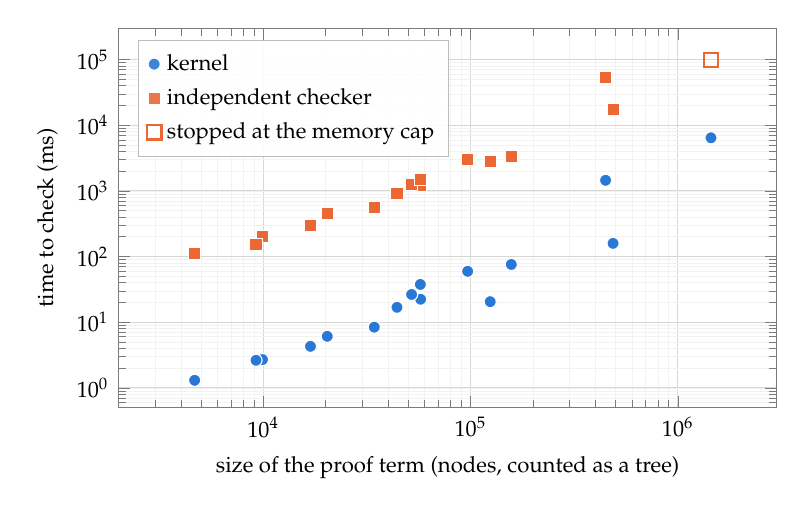
\begin{tikzpicture}
\begin{axis}[width=0.82\linewidth, height=6.4cm, xmode=log, ymode=log, xlabel={size of the proof term (nodes, counted as a tree)}, ylabel={time to check (ms)},
  xmin=2e3, xmax=3e6, ymin=0.5, ymax=3e5, grid=both, major grid style={rulegrey!60, line width=0.3pt}, minor grid style={rulegrey!20, line width=0.2pt},
  axis line style={ink!60}, tick style={ink!60}, tick label style={font=\footnotesize}, label style={font=\footnotesize},
  legend style={at={(0.03,0.97)}, anchor=north west, font=\footnotesize, draw=rulegrey, fill=white, fill opacity=0.9, text opacity=1, row sep=1pt, inner sep=3pt}, legend cell align=left]
\addplot[only marks, mark=*, mark size=2.2pt, color=cblue, mark options={draw=white, line width=0.4pt}] coordinates {\scatterKernel};
\addlegendentry{kernel}
\addplot[only marks, mark=square*, mark size=2.2pt, color=corange, mark options={draw=white, line width=0.4pt}] coordinates {\scatterIndep};
\addlegendentry{independent checker}
\addplot[only marks, mark=square, mark size=2.6pt, color=corange, mark options={line width=0.9pt}] coordinates {\scatterIndepCap};
\addlegendentry{stopped at the memory cap}
\end{axis}
\end{tikzpicture}
\caption{The cost of trusting a proof: time to check \chkSampled{} reference proofs of the problem bank, sampled evenly by length, with the kernel and with the independent checker, against the size of the proof term.
  Both axes are logarithmic.
  The hollow marker is the time at which the independent checker stopped, at its memory cap, without a verdict.}
\label{fig:trust}
\end{figure}

\paragraph{Latency of the environment.}
\Cref{tab:latency} gives percentiles of the operations of the environment, taken from the instrumented runs of the blind search and of a uniformly random policy on \blindProblems{} problems of the bank that have reference proofs, evenly spaced in length; \cref{app:probes} gives the probes by kind of action.
These are the costs of the engine on the actions that these two simple procedures try; a trained policy would try other actions, in other proportions.
\Cref{app:probes} shows that the budget does real work: of the \applyProbes{} \code{APPLY} probes, \applyFuel{} (\applyFuelShare\,\%) ended with the budget spent and not with an answer, and the budget bounds what such a probe can cost whatever the goal and whoever asks.
The slowest probe of the \probeN{} took \probeMax\,ms (a \code{REFINE}, which supplies a term with holes); the slowest \code{APPLY} probe took \applyMaxMs\,ms.

\begin{table}[t]
\centering\tabfont
\begin{tabular}{@{}lrrrr@{}}
\toprule
operation & $n$ & median (ms) & 90th (ms) & 99th (ms)\\
\midrule
probe of an action & \probeN & \probeMed & \probeNinety & \probeNinetyNine\\
menu of a goal (mean \menuMeanOpts{} options) & \menuN & \menuMed & \menuNinety & \menuNinetyNine\\
start of an episode on a problem & \startN & \startMed & \startNinety & \startNinetyNine\\
replay of one recorded action & \replayN & \replayMed & \replayNinety & \replayNinetyNine\\
one decision of the Gymnasium interface & \decN & \decMed & \decNinety & \decNinetyNine\\
\bottomrule
\end{tabular}
\caption{Latency of the operations of the environment on the problem bank (milliseconds).
  Probes, menus, starts and replays are those of the blind search and a uniformly random policy on \blindProblems{} problems; decisions are those of the instrumented Gymnasium loop with uniformly random legal choices.}
\label{tab:latency}
\end{table}

\paragraph{Throughput.}
\Cref{tab:throughput} gives rates on one core.
The engine, driven directly by the blind search, performs \blindProbesPerS{} probes per second (a range of \blindProbesMin{} to \blindProbesMax{} over two passes), and a problem takes \blindSecPerProblem\,s of its budget of \benchProbeBudget{} probes; the search solves none of the \blindProblems{} problems within that budget, and is a baseline for the cost of the machinery, not for difficulty.
The time is divided as follows (an instrumented pass, which costs \blindOverhead{} times the plain one and changes no outcome): \blindTacticShare\,\% in the tactics that carry out the actions, \blindProbeShare\,\% in the rest of the probes (checkpoint, settling, rewind), \blindMenuShare\,\% in listing menus.
Through the Gymnasium interface with uniformly random legal choices, the environment makes \gymDecPerS{} decisions per second; \gymAssemblerShare\,\% of the time is spent in the assembler that builds the questions and the options and \gymFeaturesShare\,\% in the features, while probes, the tactics that carry them out, episode starts and replays together take \gymEngineShare\,\% and menus \gymMenuShare\,\% (a profiled pass of \decN{} decisions).
A probe happens only when an action is complete, which under random choices takes \decPerProbeGym{} decisions on average in this pass, so the interface makes only \gymProbesPerS{} probes per second on this path; the same random policy driven for \uniLimitS{} seconds on each of the \blindProblems{} problems makes \uniDecPerS{} decisions, takes \uniActPerS{} actions and probes \uniProbesPerS{} times per second, \decPerProbeUni{} decisions to a probe, with \uniAssemblerShare\,\% of the time in the assembler.
The cost of a decision is therefore the cost of the Python layer that assembles it, and not of the kernel or the engine; this is where a faster implementation of the interface would gain.

\begin{table}[t]
\centering\tabfont
\begin{tabular}{@{}>{\raggedright\arraybackslash}p{6.4cm}lr@{}}
\toprule
workload (one core, unless said) & unit & rate\\
\midrule
blind search through the engine (\blindProblems{} problems) & probes per second & \blindProbesPerS\\
uniformly random choices through the Gymnasium interface & decisions per second & \gymDecPerS\\
\quad the same, driven for \uniLimitS\,s on each of the \blindProblems{} problems & decisions / actions / probes per second & \uniDecPerS\ / \uniActPerS\ / \uniProbesPerS\\
blind search in forked workers: one worker & probes per second & \wkOneRate\\
\quad two workers & probes per second & \wkTwoRate\\
\bottomrule
\end{tabular}
\caption{Throughput of the stack on the problem bank.
  The worker rows are of a different workload, the evaluation harness on \wkTasks{} tasks with a budget of 100 probes each (\wkProbes{} probes in all), and are not comparable with the first; they measure scaling and not peak speed.}
\label{tab:throughput}
\end{table}

\paragraph{Scaling, memory, determinism.}
With the world built once and shared by forked workers, two workers on the two cores finish the same \wkTasks{} tasks in \wkTwoSec\,s against \wkOneSec\,s for one, a speed-up of \wkSpeedup{} and an efficiency of \wkEff.
The memory of the pair, counted as proportional set size (what the processes cost together, where summing their resident sets would count the shared world again for each), is \wkPSS\,MB; the world of the bank (\bankGlobals{} globals, \bankProblems{} problems) is built in \bankWorldSecB\,s and peaks at \bankRSSnoTorch\,GB (\bankRSSTorch\,GB, and \bankWorldSec\,s, in the run with PyTorch loaded); of the build, \kernelShare\,\% of the time (\kernelSecInWorld\,s) is spent in the kernel's checked entry points, which received \kernelCallsInWorld{} declarations, and the rest in the Python layer that runs the tactics which construct the proofs.
Nothing is claimed beyond two workers: the machine has two cores.
The result rows of the three runs (in process, one worker, two workers) agree on every field that is not a measurement of time, for all \detTasks{} tasks and with none left out for coming near the time limit; their outcome digest is \code{\detDigest}, the same on any machine that finds the same proofs after the same number of probes.
The world of the libraries has the same digest of the names and types of its globals, \code{\worldDigestShort\ldots}, in both runs of the build.

\paragraph{Micro-benchmarks.}
A call across the Python--C++ boundary costs \ffiNsA\,ns / \ffiNsB\,ns; a checkpoint followed by a rewind of an empty region \rewPairNsA\,ns / \rewPairNsB\,ns; building a node, \nodeBuildNsA\,ns / \nodeBuildNsB\,ns from Python; and rewinding after about \rewNodes{} nodes were allocated \rewindUsA\,\textmu s / \rewindUsB\,\textmu s, or \rewindNsNodeA\,ns / \rewindNsNodeB\,ns per node.
Binary numerals are evaluated by reduction in the kernel: a product of a \prodSmallBitsA-bit and a \prodSmallBitsB-bit numeral is decided in \prodSmallMsA\,ms / \prodSmallMsB\,ms, and one of \prodLargeBitsA{} by \prodLargeBitsB{} bits in \prodLargeMsA\,ms / \prodLargeMsB\,ms.

\paragraph{What the measurements do not show.}
They are of one machine with two virtual cores, and a larger machine would change the absolute numbers and, above two workers, the scaling.
The workloads are a blind search and a random policy, and the latency of a trained policy's actions was not measured.
The sample of reference proofs for the cost of trust is \chkSampled{} of \proofsProved{}.
No figure here is compared with a figure for another system.

\subsection{How it differs from other systems}\label{sec:related}

We contrast design choices and give no speed comparison: the published figures of other systems are for other tasks on other hardware, and a fair comparison would formalise the same statements in each system and time both on one machine, which we have not done.

\paragraph{Learners attached to general-purpose assistants.}
CoqGym and GamePad (Coq), HOList (HOL Light), lean-gym, LeanDojo, Pantograph and the Kimina Lean Server (Lean) connect a learner to an existing proof assistant that runs as a separate process, and exchange text or serialised terms with it \citep{yang19,huang19,bansal19,leangym,yang23,aniva24,dossantos25}.
What this gives a learner that \ITP\ cannot give is the assistant's libraries of formalised mathematics, its automation, its community, and a kernel with a long record.
Much of the engineering of these systems goes into making the interface dependable; LeanDojo, Pantograph and the Kimina server are in part that.
\ITP\ draws the boundary elsewhere: the environment is in the process of the kernel, a state is a value that can be checkpointed, and an action is data and not syntax.
The price is the one listed in \cref{sec:properties}.

\paragraph{Purpose-built systems.}
INT, an environment and a generator of problems for inequalities, Peano, a dependently typed environment with a finite action space, and Minimo, which conjectures and proves in Peano, are environments built for learning and not interfaces to an existing assistant \citep{wu21,poesia23,poesia24}.
\ITP\ shares the aim and is closest to Peano in using dependent types and a finite menu of actions.
Its own choices are a calculus with inductive families, quotients and proof irrelevance (\cref{sec:theory}), a deterministic work budget in the kernel, a second checker and a mutation catalogue (\cref{sec:testing}), a typed term builder with which an agent says arbitrary well-typed terms (\cref{sec:env}), and a bank of competition problems with a family-disjoint split.
Hindsight relabelling on proof search trees is used by Minimo, and the idea is hindsight experience replay \citep{andrychowicz17}; we use it for the same purpose and claim nothing for it.

\paragraph{Trust.}
The kernel of Lean is small too; its type theory has been analysed formally \citep{carneiro19}, and an independent implementation of its kernel exists \citep{carneiro24}.
We do not claim a more trustworthy kernel.
The claim is narrower: the whole stack up to the action interface is small enough to be tested as a unit, by mutation among other means; the cost of every call is a deterministic budget; and a second implementation of the specification is part of the repository (\cref{sec:testing}).

\paragraph{Learners that use text.}
Language-model provers \citep{polu20,han22,polu23,lample22,jiang23,xin24,xin25,ren25,lin25,hubert25} and benchmarks such as miniF2F \citep{zheng22} work on the surface syntax of Lean, Metamath or Isabelle.
\ITP\ has no surface language, so these models and corpora do not transfer to it; its interface is aimed at policies that read tokens of goals and choose among options.
A problem bank of \bankProblems{} statements is small beside these benchmarks; what it offers is five levels of difficulty, a tier of statements without proofs that a prover is asked to find, and splits that keep the problems of a family together.

\section{Limitations}\label{sec:limits}

This section collects what the system does not do and what the evidence does not show.
It is organised by layer.
Where the log of findings (\cref{tab:findings}) has an entry, its number is given.
The log holds \findNumbers{} findings; \findOpen{} are open: F28 (conversion), F61 (the assembler of the policy interface), F67 (the time of the independent checker), and F70, which records a measurement of an early learner on an earlier version of the bank and not a defect of the system.

\subsection{The calculus}

\paragraph{Universes.}
There is no cumulativity and there is no universe polymorphism (\cref{sec:syntax}).
A definition used at two levels is written twice, and a term of one level is used at another by an explicit construction.
The eleventh kind of node, meant for level parameters, is not used.

\paragraph{Inductive types and recursion.}
A declaration is of one family (A6 of \cref{sec:ind}): there are no mutual families, no occurrence of the family nested in an argument of another (\code{List Bad}), no coinductive types, and no inductive--recursive or inductive--inductive definitions.
Recursion is structural on one argument of one family, with no mutual recursion; well-founded recursion is not a primitive.
Pattern matching on an indexed family is the kernel's \code{match} with index forcing (\cref{sec:ind}), which is first-order: it solves a field that stands alone at an index position, compares a field met twice, matches equal constructors, refutes two different ones, and declines everything else; equations between indices that need computation to solve are left to the user, and a refuted branch must still be written.
The argument that the forcing is sound is not formalised, and it is the most delicate part of the kernel.
Discrimination and injectivity lemmas are generated for families without indices or parameters only, there is no heterogeneous equality, and \code{cases} does not use them by itself (F2b).

\paragraph{Conversion.}
Conversion has $\eta$ for functions and for nothing else; there are no records, and no $\eta$ for the unit type.
Definitional proof irrelevance holds only in the Prop configuration, and the calculus has uniqueness of identity proofs there, so it is not a setting for univalent development.
The decision procedure is incomplete and not transitive on stuck case analyses (F28): two terms that each convert to their own normal form can fail to convert to each other, so that \code{exact} or \code{apply} can miss an equality that normalising both sides exposes.
The failure is in the safe direction, since a positive answer is always justified by evaluation.
Conversion is exponential in the depth of a shared term whose two sides unfold differently (F29); the work bound turns the blow-up into an exhausted budget, and the root cause is open.
A fixpoint is unfolded at any argument and not only at a constructor (F23), which is mitigated for the proofs that the tactic layer builds and remains a difference from the specification (\cref{sec:conv}).

\paragraph{Axioms, language, libraries.}
One axiom is shipped, excluded middle; the quotient rule is part of the kernel, and the integers depend on it (\cref{sec:quot}).
The audit of a theorem lists the axioms and quotient constants it depends on.
There is no surface language: a statement is a Python expression over the kernel's term builder, and there are no implicit arguments or coercions for the author, no type classes, no notation mechanism beyond infix names, and no module system.
The libraries (\libGlobals{} declarations, \cref{tab:libs}) cover the naturals, integers and some number theory; there are no real numbers, no algebraic structures, and no geometry or combinatorics.

\paragraph{Metatheory.}
Subject reduction, strong normalisation and consistency are not proved for the calculus as implemented, and no part of its metatheory is mechanised (\cref{sec:meta}).
The two deviations of \cref{app:deviations} are places where the implementation is weaker than the specification it was written against.
The second can be exploited: in a world with excluded middle and propositional extensionality as axioms, a family that the kernel admits yields a proof of $\sy{False}$, which the kernel and the independent checker both accept (\cref{lst:dev-exploit}).
We know of no exploit of the first, and we have not proved that there is none.
Neither deviation is repaired in the version of the repository that holds this report.
Neither is reachable from the environment, whose actions can neither declare a family nor say a \code{match}; both are reachable from the Python interface of the kernel, which is what a library author uses, and the exploit also needs an axiom that no shipped library assumes.

\subsection{Trust and testing}

\paragraph{Soundness is tested, not proved.}
The trusted base is the kernel (\locKernelHeader{} lines of header and \locBindings{} of bindings) and the entry points that guard it, the C++ compiler and the Python interpreter that call it.
The evidence that it is sound is the apparatus of \cref{sec:testing}, which finds defects and cannot show their absence.
Its second checker (\locchecker{} lines) is a re-implementation from the same specification by the same author, so it does not catch a flaw in the specification or a misreading that both share, and it does not re-check the admission of inductive families (D2 of \cref{app:deviations}), which is why it accepts the proof of $\sy{False}$ of \cref{lst:dev-exploit}.
The mutants are written by the author of the code and measure the tests against the faults that the author can imagine, and the \mutEquiv{} equivalent mutants are the author's judgement.

\paragraph{The independent checker is slow.}
It takes about \indOverKernel{} times the kernel's time over the libraries, between \chkRatioMin{} and \chkRatioMax{} times on the sample of reference proofs, and it needed more than \chkCapMB\,MB on one proof, where it stopped without a verdict.
The log records case-enumeration proofs for which it takes minutes (F67), which the gates check with the independent checker only on request.
It is a witness for a finished proof, not a component of a loop.

\paragraph{What was and was not run for this report.}
The gates, the sanitizer run, the library and environment measurements, and the listings were run at the commit of the report on one machine: Linux, x86-64, two virtual cores, \mCompiler.
The three listings of \cref{app:d2} that prove $\sy{False}$ and check the proof in Lean were added afterwards and run on a kernel with the same digest; the two in Lean were run with Lean 4.15.0.
The campaign of falsification by fuzzing (\code{make soundness}), a single pass of the whole mutation catalogue against the final commit, the gates run with the sharing tables of the kernel bypassed (\code{ITP\_VERIFY\_MEMO=1}), the long gates of the bank under the sanitizers, the leak detector of the sanitizer, and other platforms and compilers were not run; the repository contains the commands for each.
The measurements of cost are of this machine.
The counts and digests are properties of the code, and the times are not.

\paragraph{Budgets.}
The work bound of the kernel counts evaluation steps, and the tactics that compute in Python before the kernel sees anything have bounds of their own.
Three places where a bound was missing were found by long runs and not by any gate (F86, F87, F90), and we know of no argument that there are no others.

\subsection{The environment and the bank}

\paragraph{The interface.}
An episode acts on the first open goal; there is no choice of goal and no tactic combinator, and a proof is a sequence of single actions.
The automation is the decision procedures for polynomial arithmetic over the naturals and the integers (\code{ring}, \code{linarith}, \code{nlinarith}, \code{linear\_combination}), enumeration over an interval, and rewriting; there is no general-purpose simplifier with a lemma database that grows, no SMT back end, and no tactic for the arithmetic of the reals.
A term with \code{match} or \code{let} cannot be said to the typed builder, which concerns two proofs of the libraries and the statement of functional extensionality, and a lemma above the premise limit cannot be said.
The assembler, the policy-facing interface, says \asmSaid{} of the \asmActions{} actions of the \asmProofs{} recorded proofs of the dataset (the reference proofs of the bank in both regimes, and the libraries' proofs), at \asmMsPerAction\,ms an action.
It cannot say the other \asmMissing{}: \asmPrefixMissing{} in the reference proofs of the bank in the regime that offers every earlier global, \asmStrictMissing{} in the second proofs of the strict regime, and \asmLibMissing{} in the libraries.
They are of the kinds \asmMissingKinds{}, and in each of them some token that the action needs is not among the options offered at that point.
The log of findings (F61) attributes the failures that it had counted to steps whose terms fit their holes only up to computation, which the matcher of the typed builder does not see through; that entry was written at an earlier state of the repository and its figures do not match these, and we have not classified the present failures further.
A policy trained on the recorded actions would not meet these, and a measure of how often it can reproduce a recorded proof is bounded by the fraction that the assembler can say.
The recorder replays 453 of the 459 recorded proofs of the libraries, and the six that it does not are named in a gate.
In the prefix regime a problem with a helper on the menu can be a single action, which measures the use of a lemma and not the finding of an idea; the strict regime hides the helpers, and only the problems with a self-contained reference proof have one.

\paragraph{The bank.}
It is small (\bankProblems{} problems) and tilted toward the easy end.
\Cref{tab:bank} gives the levels: \bankLevelsLowProved{} of the \proofsProved{} problems with a reference proof are of levels 1 to 3, and of the \bankLevelFiveTotal{} problems of level 5 one has a proof.
Of the \bankImoLike{} problems from the IMO, its shortlist and the APMO, \bankImoLikeProved{} have a proof; the others are statements, with exhaustive evidence on small ranges that they are true.
Of the problems, \bankOrigContest{} are formalised as in a contest, \bankOrigAdapted{} are changed to fit the vocabulary (integers instead of reals, one part of several), \bankOrigStyle{} are written for the bank in the manner of a contest and are not contest problems, and \bankOrigFolklore{} are classical facts and exercises; the texts of the AIME problems are paraphrased.
The topics are arithmetic, algebra and number theory (\bankTopicNT{} problems carry the number-theory tag); \bankTopicCombinatorics{} are tagged combinatorics and none is geometry.
That a statement says what its problem says is checked by evaluation on windows of small values against an executable reading written by the person who formalised it, and no second reader has recorded a verdict; a misreading shared by the statement and its executable reading is invisible to every check.
The split is by family, so that the test problems are not restatements of training problems, but \bankSplitTest{} problems in a test split, eight of them statements without proofs, are a small test.

\begin{table}[t]
\centering\tabfont
\begin{tabular}{@{}cccc@{}}
\toprule
level & with a reference proof & statement only & all\\
\midrule
\bankLevelRows
\bottomrule
\end{tabular}
\caption{The problems of the bank by level (how much thinking a problem asks for, not how long its proof is) and by whether a kernel-checked reference proof exists.
  The counts are read from the released dataset file.}
\label{tab:bank}
\end{table}

\paragraph{Hindsight and throughput.}
Hindsight returns the sub-theorems of a proof tree that can be made exact; those that cannot are dropped and counted, so the yield on a given attempt is less than the number of its solved sub-goals.
The interface is in Python, and a decision costs the cost of the assembler (\cref{sec:measure}); the throughput of a decision is therefore far from the throughput of the kernel.
Scaling was measured to two workers on a machine with two cores.
No GPU or accelerator is involved in the environment, and none was measured.

\paragraph{No learning.}
The report contains no experiment in which a policy was trained on the environment, and claims nothing about what a learner would achieve with it.
\Cref{sec:why} describes properties of the interface and what they cost; whether they help a learner is the subject of future work, and the comparison with other systems is of design and not of speed.

\section{Conclusion}\label{sec:conclusion}

We have described \ITP, a proof assistant built to be the environment of a learning system: a dependent type theory with inductive families, an impredicative bottom universe, quotients and a structural guard, decided by a C++ kernel of about \locKernelHeader{} lines; a Miller-pattern unifier and certificate-checked decision procedures for polynomial arithmetic; a second, independent checker; and a layer that turns the assistant into an environment, with a finite menu of actions and a typed term builder for the rest, probes that try an action and take it back, work counted in kernel steps, exact hindsight, a bank of \bankProblems{} problems, and a Gymnasium interface with no text in the loop.

What the evidence supports is modest and concrete.
A probe of an action costs a median of \probeMed\,ms and a decision of the Gymnasium interface \decMed\,ms on one core of a two-core machine; the kernel checks the median reference proof of the bank in \chkKernelMedianMs\,ms, so that the verdict can be had for every finished proof, and the independent checker confirms it about \chkRatioMedian{} times more slowly, as a witness.
The soundness of the kernel is tested, not proved, by a frozen reference kernel run in lockstep, a second checker, canaries, a fuzzer, \mutTotal{} mutants, sanitizers and a log of \findNumbers{} findings.
The testing also reached its own limits: writing the rules down for this report turned up two places where the kernel checks less than the usual conditions on a motive and on the positivity of a family (\cref{app:deviations}); the second checker, written from the same specification, shares the first omission in part and does not examine the second.
The second omission can be exploited: with excluded middle and propositional extensionality added to a world, a family that the kernel admits gives a proof of $\sy{False}$ that both checkers accept (\cref{app:d2}).

What the evidence does not show is whether a learner profits.
The report has no learning experiment, and its claims about the design are claims about an interface: a verdict the proposer cannot influence, states that can be restored, actions that are well formed by construction, a cost that is a function of the task, and failures that yield theorems.
Whether these properties help is an empirical question that needs a fixed protocol, an untrained control, and a budget measured in the unit that the environment provides; the environment is meant to make that experiment cheap to run and its outcome checkable.

\paragraph{Future work.}
The two deviations of \cref{app:deviations} are not repaired in this version and should be, in the kernel, with a gate for each (for the second, the proof of $\sy{False}$ of \cref{lst:dev-exploit} must fail at the declaration of \code{R}), and the independent checker should re-check the admission of inductive families.
The remaining gaps of the calculus, universe polymorphism, mutual and nested families and a real-number library, bound the mathematics that the bank can contain; the bank itself needs a second reader of its statements and proofs for its hard tier.
A faster implementation of the policy interface would move the throughput of a decision toward that of the kernel.
Part of the metatheory, starting with the guard and the forcing of indices, could be mechanised.
And the environment should be used: to train and to compare learners on the bank and on synthetic theorems, against an untrained control, with the budgets of this report.

\subsection*{Availability and reproducibility}\label{sec:availability}

The code, the dataset of the problem bank, the sources of this report and the scripts that produced its numbers are in one repository at commit \mCommit{} (\reporturl); a snapshot is archived with the report (\reportdoi), under the licence \artifactlicense.
The directory \code{preprint/} of the repository holds the sources of the report (\code{src/}), the bibliography, the measurement scripts, the listings and their outputs, and the raw measurements as JSON and logs; \code{python3 -I preprint/build.py} regenerates every macro that holds a number, and then the PDF, from them.
The scripts and their costs on the machine of \cref{sec:measure} are: \code{measure.py}, the library chain, its re-check by the kernel and by the independent checker, and the micro-benchmarks (about three minutes); \code{measure\_check.py}, the cost of trusting a sample of reference proofs (about ten minutes, 2\,GB); \code{src/python/experiments/exp\_bench.py}, the latency and the throughput of the environment (a few minutes after the world is built); \code{measure\_assembler.py}, the round trip of the policy interface; \code{measure\_gates.py}, the gates named in \cref{tab:testing} and the sanitizer run; and \code{run\_listings.py}, the listings of \cref{sec:usage} and \cref{app:deviations} (those in Lean need a Lean~4).
The code, the dataset and the world are identified by digests so that a rerun can be compared with ours: the digest of the directory of the kernel's sources (\code{src/c++/hybrid}) is \code{\kernelDigest}, that of the names and types of the \libGlobals{} globals of the library world is \code{\worldDigestShort\ldots}, and that of the outcomes of the benchmark tasks is \code{\detDigest}.
The counts of this report (lines, declarations, mutants, findings, problems, proofs) are read from the files of the repository and do not depend on the machine; the times do.

\appendix

\section{Two deviations of the kernel}\label{app:deviations}

The two deviations below were found while the rules of \cref{sec:theory} were written down from the code, by reading it and by probing it; no gate found either.
The second checker shares part of the first omission (it does not compare the binder types of a motive either, though it does require the motive to end in a sort) and does not examine the admission of a family at all (\cref{sec:indep}).
The second deviation can be exploited: once excluded middle and propositional extensionality are added to a world, a family that the kernel accepts yields a proof of $\sy{False}$, which the kernel and the second checker both accept (\cref{app:d2}).
Neither deviation is repaired in the version of the repository that holds this report: the sources of its kernel are those of commit \mCommit{}, the commit of the measurements (digest \code{\kernelDigest}).
Each deviation has a listing in the supplementary material that reproduces it (\code{preprint/listings/dev\_motive.py} and \code{dev\_positivity.py}), and the exploit has three more, one in the system and two in Lean (\code{dev\_exploit.py}, \code{dev\_lean\_decl.lean} and \code{dev\_lean\_false.lean}); \Cref{lst:dev-motive,lst:dev-pos,lst:dev-exploit,lst:dev-lean-decl,lst:dev-lean-false} show them with the output of a run on that kernel.

\subsection{D1: the motive of a match is checked for its shape}\label{app:d1}

The usual rule for $\matchx{s}{M}{\vs b}$ with $s : I\,\vs a$ requires $M : \Pi(\vs y{:}\vs Y)(z{:}I\,\vs y).\,S$, where $\vs Y$ are the index types of $I$ at the parameters of $s$ and $S$ is a sort.
The kernel's check of an explicit motive (\code{verify\_motive\_shape}) infers the type of $M$, evaluates it, and checks that it is a chain of $|\vs a|+1$ products.
It does not compare the binder types with $\vs Y$ and $I\,\vs y$, and it does not require that what follows the last product is a sort (the message of its error speaks of a chain ``ending in a sort'', but the code reads the level of the sort only when the value is one, and otherwise goes on).

\lstfile[firstline=3]{Deviation D1: three motives, two of which the kernel does not refuse.}{lst:dev-motive}{listings/dev_motive.py}
\lstinputlisting[style=out]{listings/dev_motive.out}

In case (a) the motive abstracts over a second data type and is applied, in the types of the branches, to terms of \code{Nat}; the kernel infers a type, the checked entry point accepts the declaration, and the independent checker accepts it too: it checks the number of products and that the codomain is a sort, and does not compare the binder types either.
In case (b) the codomain of the motive is a term and not a sort; the kernel infers a type for the match, and the checked entry point refuses the declaration because that type is not a type.
Nothing of (b) remains for the independent checker to re-check, and its source states the condition on the sort that the kernel's shape check lacks.
Case (c), a motive with no binder, is refused.

\paragraph{Exposure.}
The function form of \code{match} of the authoring layer builds the motive's binder from the type of the scrutinee, and cannot produce (a); an indexed family needs the explicit form, and so does any code that builds terms directly.
The actions of the environment cannot say a \code{match} (\cref{sec:env}).
We have not scanned the matches of the shipped terms for ill-formed motives, and we do not know whether (a) can be exploited to derive a contradiction.
A motive that analyses its argument would be applied to terms of the wrong type, and the untyped evaluator would reduce such an application by the shape of the term.
\paragraph{Repair.}
Compare each binder type with the expected one by conversion, and require the codomain to be a sort, in \code{verify\_motive\_shape}; add the cases of the listing to the gates.

\subsection{D2: strict positivity does not look in the indices}\label{app:d2}

Condition A5 of \cref{sec:ind} examines the types of the fields: a field type is accepted if the family does not occur in it, or if it is a product whose domain does not contain the family and whose codomain is accepted, or if its head is the family.
Nothing is examined inside the arguments of that head, and nothing inside the result indices of the constructor.
The usual conditions for indexed families exclude the family from both \citep{dybjer94,paulin93}.

\lstfile[firstline=3]{Deviation D2: a negative occurrence in the index of a recursive field, and in a result index.}{lst:dev-pos}{listings/dev_positivity.py}
\lstinputlisting[style=out]{listings/dev_positivity.out}

The family \code{Q} of \cref{lst:dev-pos} has a field of type $\Fam{Q}\,(\Fam{Q}\,A\to\sy{False})$, in which $\Fam{Q}$ occurs to the left of an arrow inside an index; \code{R} has $\Fam{R}\,A\to\sy{False}$ as a result index.
Both are accepted; the control, with the family to the left of an arrow in a field, is refused.
The independent checker re-checks the declarations of the constants and finds nothing, because it does not re-check the admission of inductive families (\cref{sec:indep}).

\paragraph{An exploit.}
The family \code{R} yields a proof of $\sy{False}$ once two standard classical axioms are added to the world: excluded middle, $\forall P{:}\Prop.\;P\lor\lnot P$, and propositional extensionality, $\forall P\,Q{:}\Prop.\;(P\leftrightarrow Q)\to P=Q$.
Write $E\,x$ for $\Fam{R}\,x\to\sy{False}$.
The constructor gives $\Fam{R}\,(E\,B)$ for every proposition $B$, and, since it is the only constructor, the elimination of an inhabitant of $\Fam{R}\,x$ into a proposition gives $\exists B.\;E\,B=x$ (\code{R\_inv}).
So $\Fam{R}\,x$ is inhabited exactly when $x$ is a value of $E$; hence $E\,x$ is refuted when $x$ is a value of $E$ (\code{K1}) and holds when it is not (\code{K3}), and neither lemma uses an axiom.
With the two axioms every proposition is equal to $\sy{True}$ or to $\sy{False}$, so $E$ has at most two values, and each of the cases for $E\,\sy{False}$ and $E\,\sy{True}$ contradicts ``$E\,x$ holds exactly when $x$ is not a value of $E$''.
\Cref{lst:dev-exploit} carries this out through the checked entry point of the kernel, in the base library of the repository extended by the two axioms and the family; it ends with \code{boom : False}.
The audit of \code{boom}, the counterpart of the \code{\#print axioms} of Lean, lists the two axioms and no others, and the independent checker re-checks every declaration of the world, \code{boom} included, and finds no problem, since it does not look at the admission of \code{R}.

\lstfile[firstline=3]{Deviation D2 exploited: a proof of \texttt{False} from \texttt{R}, excluded middle and propositional extensionality.}{lst:dev-exploit}{listings/dev_exploit.py}
\lstinputlisting[style=out]{listings/dev_exploit.out}

The fault is in the rules of \code{R}, and not in the encoding of the proof or in the axioms.
The kernel of Lean 4.15.0, which applies the usual positivity condition, refuses \code{R}, and \code{Q} and the control as well (\cref{lst:dev-lean-decl}).
If the constructor of \code{R} and the elimination into propositions that its declaration would give are postulated as axioms, Lean proves $\sy{False}$ from \code{Classical.propComplete}, the statement that every proposition is equal to $\sy{True}$ or to $\sy{False}$ (\cref{lst:dev-lean-false}; both Lean listings use the core library only).

\lstfile[language=Lean]{Lean 4.15.0 and the three families of \cref{lst:dev-pos}: its kernel refuses all of them.}{lst:dev-lean-decl}{listings/dev_lean_decl.lean}
\lstinputlisting[style=out]{listings/dev_lean_decl.out}

\lstfile[language=Lean]{Lean 4.15.0 with the rules of \texttt{R} as axioms: \texttt{False} follows from \texttt{Classical.propComplete}.}{lst:dev-lean-false}{listings/dev_lean_false.lean}
\lstinputlisting[style=out]{listings/dev_lean_false.out}

The axioms are needed for this proof.
Together they say that $\Prop$ has two elements, $\sy{True}$ and $\sy{False}$, and in a model that interprets $\Prop$ by two truth values \code{R} has no interpretation: $E$ would be a map of $\{0,1\}$ to itself with $E\,x=1$ exactly when $x$ is not in its image, and none of the four such maps is.
Both axioms are standard (Lean's core library has them, excluded middle through its axiom of choice, and the standard library of Coq offers them), and the library of this repository assumes the first.
We do not know whether the calculus with \code{R} and without the axioms is consistent, and we know of no exploit of \code{Q}.

\paragraph{Exposure.}
We read back every inductive family of the world of the bank through the kernel's term view (\code{measure\_deviations.py}): \dtwoFamilies{} families with \dtwoCtors{} constructors, of which \dtwoRecFams{} have a recursive field.
None has the family in an index of a recursive field, in a result index, or anywhere else that condition A5 rejects, so the shipped libraries and the statements of the bank are not affected.
The scan flags the two families of \cref{lst:dev-pos} and none of the families of the natural-number library, which it checks before it reads the bank.
The environment can declare neither a family nor an axiom, and the shipped libraries assume excluded middle and not propositional extensionality, so the exploit is open to the author of a library, through the Python interface of the kernel, and to no one else; the libraries, the proofs of the bank and the measurements of this report do not depend on the gap.
\paragraph{Repair.}
Reject an occurrence of the family in the arguments of a recursive occurrence and in the result indices, in the admission of the family; make the independent checker re-check admission from the stated condition; add the exploit to the gates, with the declaration of \code{R} now refused.
This repair is not applied in this version.

\section{The reference proofs checked}\label{app:check}

\Cref{tab:check} lists the \chkSampled{} reference proofs of the bank that \cref{fig:trust} plots, sampled evenly by length: the number of actions, the size of the proof term counted as a tree, the time of the kernel's check against the statement, the time of the independent checker in a child process with a cap of \chkCapS\,s and \chkCapMB\,MB, the ratio of the two times, and the memory the checker allocated beyond the world it inherited.

\begin{table}[h]
\centering\tabfont
\begin{tabular}{@{}lrrrrrr@{}}
\toprule
problem & actions & term nodes & kernel (ms) & indep. (ms) & ratio & MB\\
\midrule
\checkRows
\bottomrule
\end{tabular}
\caption{The sample of reference proofs behind \cref{fig:trust}.
  The times are those of one run on the machine of \cref{sec:measure}.}
\label{tab:check}
\end{table}

\section{Probes by kind of action}\label{app:probes}

\Cref{tab:probes} gives the latency of probes by the kind of action, for the eleven most frequent of the \probeKindsTotal{} kinds that the blind search and the random policy of \cref{sec:measure} tried, with the number of probes that ended \code{ok}, \code{refused} and \code{fuel}.
A blind search and a random policy try actions in proportions that a trained policy would not, so the table shows what each kind of probe can cost and not how often it would be asked.

\begin{table}[h]
\centering\tabfont
\begin{tabular}{@{}lrrrrr@{}}
\toprule
kind & probes & median (ms) & 90th (ms) & 99th (ms) & ok / refused / fuel\\
\midrule
\probeKindRows
\bottomrule
\end{tabular}
\caption{Probes by kind of action, from the runs of \cref{tab:latency}.}
\label{tab:probes}
\end{table}

\section{The gates}\label{app:gates}

\Cref{tab:gateindex} lists the \gatesAll{} gates with the time each took in the run for this report, on the machine of \cref{sec:measure}, two gates at a time; the machine also did other work of the report while the gates ran, so the times are indicative.
The description is the first clause of the one in \code{tests/README.md}.
\fullGatesSentence

{\tabfont\setlength{\tabcolsep}{4pt}
\begin{longtable}{@{}>{\raggedright\arraybackslash}p{1.15cm}>{\raggedright\arraybackslash}p{3.7cm}r>{\raggedright\arraybackslash}p{7.1cm}@{}}
\caption{The gates, the time of each in the run for this report, and what it protects.}\label{tab:gateindex}\\
\toprule
gate & script & s & protects\\
\midrule
\endfirsthead
\toprule
gate & script & s & protects\\
\midrule
\endhead
\bottomrule
\endfoot
\gateIndexRows
\end{longtable}}

\bibliographystyle{abbrvnat}
\bibliography{references}

\end{document}
